\documentclass[11pt,a4paper]{article}

% définition des marges du document
\setlength{\topmargin}{0cm}
\setlength{\headheight}{0.4cm}
\setlength{\headsep}{0.8cm}
\setlength{\footskip}{1cm}
\setlength{\textwidth}{17cm}
\setlength{\textheight}{25cm}
\setlength{\voffset}{-1.5cm}
\setlength{\hoffset}{-0.5cm}
\setlength{\oddsidemargin}{0cm}
\setlength{\evensidemargin}{0cm}

\usepackage[
        backend=biber,
        style=phys,  
        mcite=true,
        subentry,
        hyperref=true,
        ]{biblatex}
\addbibresource{Rapport.bib}

\usepackage{graphicx} % inclusion des figures
\usepackage{tabularx} % gestion avancée des tableaux

\usepackage{physics}
\usepackage{wrapfig}
\usepackage{amsmath} % collection de symboles mathématiques
\usepackage{amssymb} % collection de symboles mathématiques

\usepackage[utf8]{inputenc}
\usepackage[T1]{fontenc}
\DeclareUnicodeCharacter{2212}{-}

\usepackage[english]{babel}

\usepackage{siunitx}
\usepackage[version=4]{mhchem}


\usepackage{xcolor} % gestion de différentes couleurs

\definecolor{linkcolor}{rgb}{0,0,0.6} % définition de la couleur des liens pdf
\newcommand{\titou}[1]{\textcolor{red}{#1}}
\newcommand{\antoine}[1]{\textcolor{orange}{#1}}
\usepackage[ pdftex,colorlinks=true,
pdfstartview=FitV,
linkcolor= linkcolor,
citecolor= linkcolor,
urlcolor= linkcolor,
hyperindex=true,
hyperfigures=false]
{hyperref} % fichiers pdf 'intelligents', avec des liens entre les références, etc.
\usepackage{fancyhdr} % entêtes et pieds de pages personnalisés

% définition de l'entête et du pied de page
\pagestyle{fancy}
\fancyhead[L]{\scriptsize \textsc{Perturbation theory in the complex plane}}
\fancyhead[R]{\scriptsize \textsc{Antoine \textsc{MARIE}}}
\fancyfoot[C]{ \thepage}

\newcommand{\hH}{\Hat{H}}
\newcommand{\hV}{\Hat{V}}
\newcommand{\hI}{\Hat{I}}
\newcommand{\hS}{\Hat{S}}
\newcommand{\bH}{\mathbf{H}}
\newcommand{\bV}{\mathbf{V}}
\newcommand{\pt}{$\mathcal{PT}$}

\begin{document}

% Pour faciliter la mise en forme de la page du titre, on supprime l'indentation automatique en début de paragraphe
\setlength{\parindent}{0pt}

% Pas d'en-tête ni de pied pour la première page
\thispagestyle{empty}


\includegraphics[height=2cm]{logoens.eps} \hfill 
\includegraphics[height=2cm]{logoucbl.eps} \hfill 
\includegraphics[height=2cm]{logounivlyon.eps}
\vspace{0.5cm}

\begin{tabularx}{\textwidth}{@{} l X l @{} }
{\sc Licence / Master Science de la matière} & & Stage 2019-2020 \\
{\it École Normale Supérieure de Lyon} & & Antoine \textsc{MARIE} \\
{\it Université Claude Bernard Lyon I} & & M1 Chimie
\end{tabularx}

\begin{center}

\vspace{1.5cm}

\rule[11pt]{5cm}{0.5pt}

\textbf{\huge Pertubation theory in the complex plane}

\rule{5cm}{0.5pt}

\vspace{1.5cm}

\parbox{15cm}{\small
\textbf{Abstract} : \it In this work, we explore the extension of quantum chemistry in the complex plane. We observe that the physics of a quantum system is intimately connected to the position of the energy singularities in the complex plane. After a brief presentation of the fundamental notions of quantum chemistry and perturbation theory in the complex plane, we provide a historical overview of the various research activities that have been performed on the physic of singularities. Then we connect and further discuss these different aspects using the spherium model (i.e., two opposite-spin electrons restricted to remain on the surface of a sphere) as a theoretical playground. In particular, we explore various perturbative partitioning strategies and the effects of symmetry breaking on the singularity structure of the electronic energy. This provides fundamental insights on the location of these singularities in the complex plane (that one calls exceptional points) and, specifically, on the magnitude of the radius of convergence associated with the perturbative treatment.
}

\vspace{0.5cm}

\parbox{15cm}{
\textbf{Keywords} : \it quantum chemistry, perturbation theory, complex plane, spherium, exceptional points, radius of convergence, symmetry breaking
} %fin de la commande \parbox des mots clefs

\vspace{0.5cm}

\parbox{15cm}{
Internship supervisor:

{\bf Pierre-François \textsc{LOOS}}

\href{mailto:loos@irsamc.ups-tlse.fr}{\tt loos@irsamc.ups-tlse.fr} / tél. (+33) 5 61 55 73 39

Laboratoire de Chimie et Physique Quantiques

{\it 118, route de Narbonne

31062 Toulouse - France}

\url{https://www.irsamc.ups-tlse.fr/loos}
} %fin de la commande \parbox encadrant / laboratoire d'accueil

\vspace{0.5cm}

\includegraphics[height=2cm]{LCPQ_logo.pdf} \hfill 
\includegraphics[height=2cm]{LogoCNRS.eps} \hfill 
\includegraphics[height=2cm]{UPS_logo.jpg}

\end{center}

\vfill
\hfill \today

\newpage
\thispagestyle{empty}

\setlength{\parindent}{17pt}

\section*{Acknowledgments}

\tableofcontents

\newpage
\setcounter{page}{1}

%============================================================%
\section{Introduction}
\label{sec:intro}
%============================================================%

\subsection{Background}

Due to the ubiquitous influence of processes involving electronic excited states in physics, chemistry, and biology, their faithful description from first principles has been one of the grand challenges faced by theoretical chemists since the dawn of computational chemistry. 
Accurately predicting ground- and excited-state energies (hence excitation energies) is particularly valuable in this context, and it has concentrated most of the efforts within the community.
An armada of theoretical and computational methods have been developed to this end, each of them being plagued by its own flaws. 
The fact that none of these methods is successful in every chemical scenario has encouraged chemists to carry on the development of new excited-state methodologies, their main goal being to get the most accurate excitation energies (and properties) at the lowest possible computational cost in the most general context.

One common feature of all these methods is that they rely on the notion of quantized energy levels of Hermitian quantum mechanics, in which the different electronic states of a molecule or an atom are energetically ordered, the lowest being the ground state while the higher ones are excited states. 
Within this quantized paradigm, electronic states look completely disconnected from one another.
Many current methods study excited states using only ground-state information, creating a ground-state bias that leads to incorrect excitation energies.
However, one can gain a different perspective on quantization extending quantum chemistry into the complex domain.
In a non-Hermitian complex picture, the energy levels are \textit{sheets} of a more complicated topological manifold called \textit{Riemann surface}, and they are smooth and continuous \textit{analytic continuation} of one another.
In other words, our view of the quantized nature of conventional Hermitian quantum mechanics arises only from our limited perception of the more complex and profound structure of its non-Hermitian variant.
The realization that ground and excited states both emerge from one single mathematical structure with equal importance suggests that excited-state energies can be computed from first principles in their own right.
One could then exploit the structure of these Riemann surfaces to develop methods that directly target excited-state energies without needing ground-state information.

\begin{wrapfigure}{R}{0.5\textwidth}
    \centering
    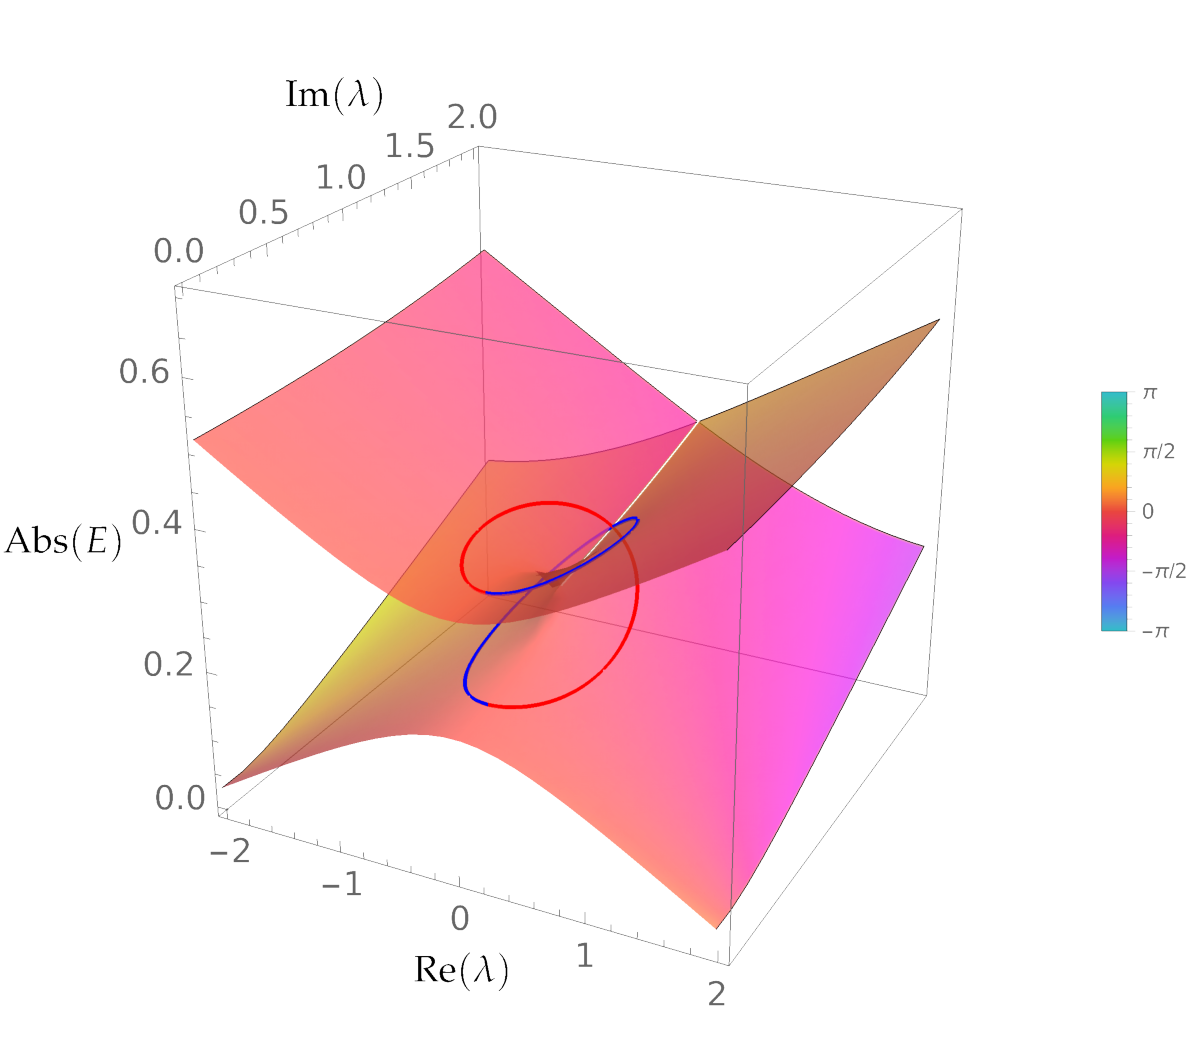
\includegraphics[width=\linewidth]{TopologyEP.pdf}
    \caption{A generic EP with the square-root branch point topology. A loop around the EP interconvert the states.}
    \label{fig:TopologyEP}
\end{wrapfigure}
By analytically continuing the electronic energy $E(\lambda)$ in the complex domain (where $\lambda$ is a coupling parameter), the ground and excited states of a molecule can be smoothly connected.
This connection is possible because by extending real numbers to the complex domain, the ordering property of real numbers is lost.
Hence, electronic states can be interchanged away from the real axis since the concept of ground and excited states has been lost.
Amazingly, this smooth and continuous transition from one state to another has recently been experimentally realized in physical settings such as electronics, microwaves, mechanics, acoustics, atomic systems and optics \cite{Bittner_2012, Chong_2011, Chtchelkatchev_2012, Doppler_2016, Guo_2009, Hang_2013, Liertzer_2012, Longhi_2010, Peng_2014, Peng_2014a, Regensburger_2012, Ruter_2010, Schindler_2011, Szameit_2011, Zhao_2010, Zheng_2013, Choi_2018, El-Ganainy_2018}.

Exceptional points (EPs) are branch point singularities where two (or more) states become exactly degenerate \cite{Heiss_1990, Heiss_1999, Heiss_2012, Heiss_2016}. 
They are the non-Hermitian analogs of conical intersections \cite{Yarkony_1996}.
Conical intersections are ubiquitous in non-adiabatic processes and play a key role in photo-chemical mechanisms.
In the case of auto-ionizing resonances, EPs have a role in deactivation processes similar to conical intersections in the decay of bound excited states.
Although Hermitian and non-Hermitian Hamiltonians are closely related, the behavior of their eigenvalues near degeneracies is starkly different.
For example, encircling non-Hermitian degeneracies at EPs leads to an interconversion of states, and two loops around the EP are necessary to recover the initial energy (see Fig.~\ref{fig:TopologyEP} for a graphical example).
Additionally, the wave function picks up a geometric phase (also known as Berry phase \cite{Berry_1984}) and four loops are required to recover the initial wave function.
In contrast, encircling Hermitian degeneracies at conical intersections only introduces a geometric phase while leaving the states unchanged.
More dramatically, whilst eigenvectors remain orthogonal at conical intersections, at non-Hermitian EPs the eigenvectors themselves become equivalent, resulting in a \textit{self-orthogonal} state \cite{MoiseyevBook}.
More importantly here, although EPs usually lie off the real axis, these singular points are intimately related to the convergence properties of perturbative methods and avoided crossing on the real axis are indicative of singularities in the complex plane \cite{Olsen_1996, Olsen_2000}.

\subsection{An illustrative example}
In order to highlight the general properties of EPs mentioned above, we propose to consider the following $2 \times 2$ Hamiltonian commonly used in quantum chemistry

\begin{equation}
\label{eq:H_2x2}
	\bH = 
	\begin{pmatrix}
		\epsilon_1	&	\lambda	\\
		\lambda		&	\epsilon_2
	\end{pmatrix},
\end{equation}
which represents two states of energies $\epsilon_1$ and $\epsilon_2$ coupled with a strength of magnitude $\lambda$.
This Hamiltonian could represent, for example, a minimal-basis configuration interaction with doubles (CID) for the hydrogen molecule \cite{SzaboBook}.

For real $\lambda$, the Hamiltonian \eqref{eq:H_2x2} is clearly Hermitian, and it becomes non-Hermitian for any complex $\lambda$ value.
Its eigenvalues are
\begin{equation}
\label{eq:E_2x2}
	E_{\pm} = \frac{\epsilon_1 + \epsilon_2}{2} \pm \frac{1}{2} \sqrt{(\epsilon_1 - \epsilon_2)^2 + 4\lambda^2},
\end{equation}
and they are represented as a function of $\lambda$ in Fig.~\ref{fig:2x2}.
One notices that the two states become degenerate only for a pair of complex conjugate values of $\lambda$
\begin{equation}
\label{eq:lambda_EP}
	\lambda_\text{EP} = \pm i\,\frac{\epsilon_1 - \epsilon_2}{2},
	\quad
	\text{with energy}	
	\quad
	E_\text{EP} = \frac{\epsilon_1 + \epsilon_2}{2},
\end{equation}
which correspond to square-root singularities in the complex-$\lambda$ plane (see Fig.~\eqref{fig:2x2}).
These two $\lambda$ values, given by Eq.~\eqref{eq:lambda_EP}, are the so-called EPs and one can clearly see that they connect the ground and excited states.
Starting from $\lambda_\text{EP}$, two square-root branch cuts run on the imaginary axis towards $\pm i \infty$.
In the real $\lambda$ axis, the point for which the states are the closest ($\lambda = 0$) is called an avoided crossing and this occurs at $\lambda = \Re(\lambda_\text{EP})$.
The ``shape'' of the avoided crossing is linked to the magnitude of $\Im(\lambda_\text{EP})$: the smaller $\Im(\lambda_\text{EP})$, the sharper the avoided crossing is.

\begin{figure}[h!]
    \centering
    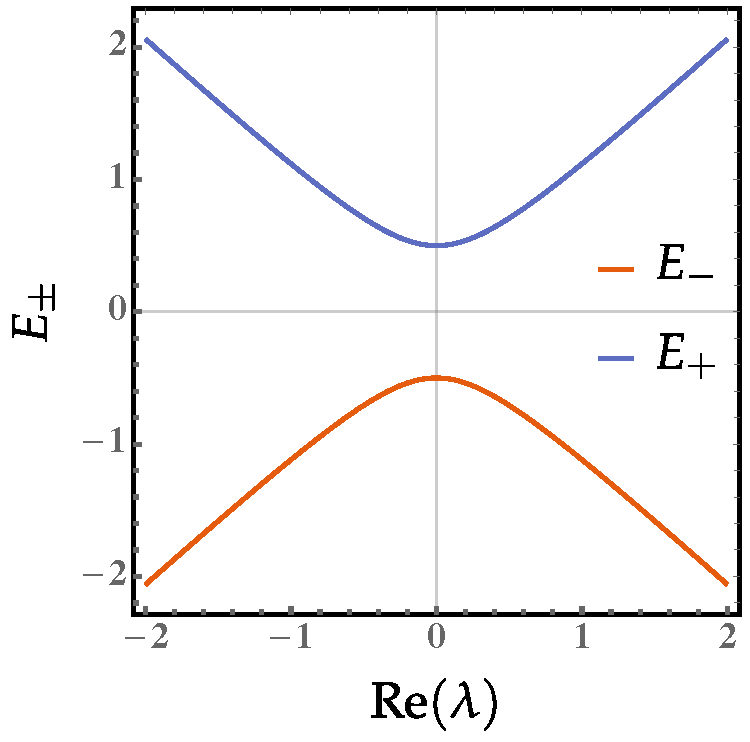
\includegraphics[width=0.3\textwidth]{2x2.pdf}
    \hspace{0.2\textwidth}
    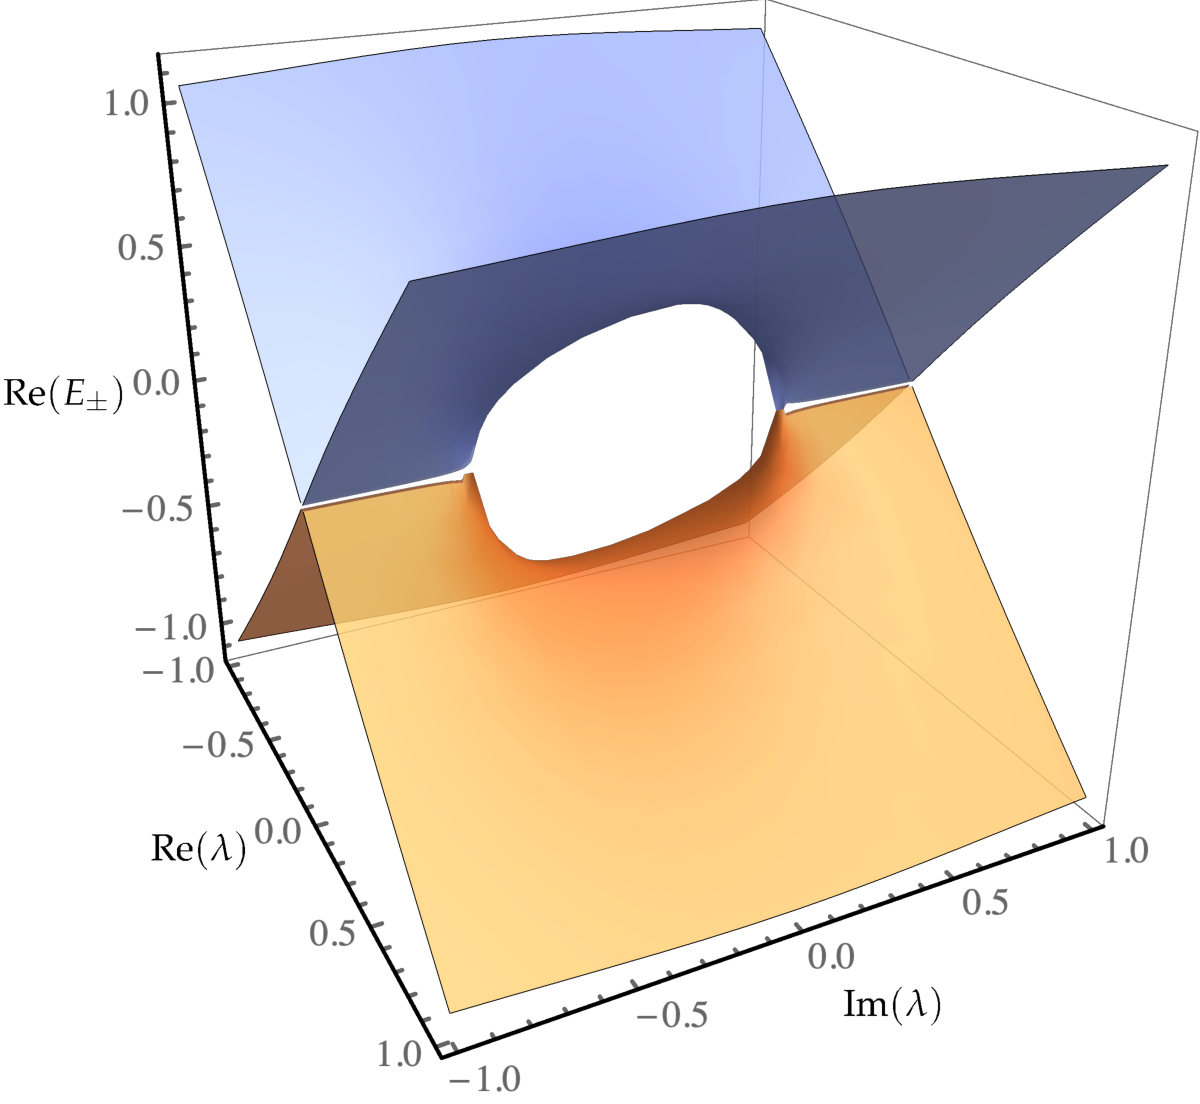
\includegraphics[width=0.3\textwidth]{i2x2.pdf}
    \caption{Energies, as given by Eq.~\ref{eq:E_2x2}, of the Hamiltonian \eqref{eq:H_2x2} as a function of $\lambda$ with $\epsilon_1 = -1/2$ and $\epsilon_2 = +1/2$.}
    \label{fig:2x2}
\end{figure}

Around $\lambda = \lambda_\text{EP}$, Eq.~\eqref{eq:E_2x2} behaves as \cite{MoiseyevBook}
\begin{equation} \label{eq:E_EP}
        E_{\pm} = E_\text{EP} \pm \sqrt{2\lambda_\text{EP}} \sqrt{\lambda - \lambda_\text{EP}},
\end{equation}
and following a complex contour around the EP, i.e., $\lambda = \lambda_\text{EP} + R \exp(i\theta)$, yields
\begin{equation}
        E_{\pm}(\theta) = E_\text{EP} \pm \sqrt{2\lambda_\text{EP} R}  \exp(i\theta/2),
\end{equation}
and we have
\begin{align}
	E_{\pm}(2\pi) & = E_{\mp}(0),
	&
	E_{\pm}(4\pi) & = E_{\pm}(0).
\end{align}
This evidences that encircling non-Hermitian degeneracies at EPs leads to an interconversion of states, and two loops around the EP are necessary to recover the initial energy.

The eigenvectors associated to the eigenenergies \eqref{eq:E_2x2} are
\begin{equation}\label{eq:phi_2x2}
\begin{split}
	\phi_{\pm}
	& = 
	\begin{pmatrix}
		(\epsilon_1 - \epsilon_2 \pm \sqrt{(\epsilon_1 - \epsilon_2)^2 + 4\lambda^2})/2\lambda 
		\\ 
		1
	\end{pmatrix}
	\\
	& =
	\begin{pmatrix}
		(\epsilon_1-\epsilon_2)/2\lambda \pm \sqrt{2\lambda_\text{EP}} \sqrt{\lambda - \lambda_\text{EP}}/\lambda 
		\\ 
		1
	\end{pmatrix},
\end{split}
\end{equation}
and, for $\lambda=\lambda_\text{EP}$, they become
\begin{align}
	\phi_{\pm} & = \begin{pmatrix} -i \\ 1\end{pmatrix},
	&
	\phi_{\pm} & = \begin{pmatrix} i \\ 1\end{pmatrix},
\end{align}
which are clearly self-orthogonal, i.e., their norm is equal to zero. 
%Using Eq.~\eqref{eq:E_EP}, Eq.~\eqref{eq:phi_2x2} can be recast as
%\begin{equation}\label{eq:phi_EP}
%\phi_{\pm}=
%\end{equation}
As branch point (square-root) singularities, EPs inherit their topology from the multi-valued function $\sqrt{\lambda - \lambda_\text{EP}}$. 
Then, if the eigenvectors are properly normalized, they behave as $(\lambda - \lambda_\text{EP})^{-1/4}$, which gives the following pattern when looping around one EP:
\begin{align}
	\phi_{\pm}(2\pi) & = \phi_{\mp}(0),
	&
	\phi_{\pm}(4\pi) & = -\phi_{\pm}(0), 
	&
	\phi_{\pm}(6\pi) & = -\phi_{\mp}(0),
	&
	\phi_{\pm}(8\pi) & = \phi_{\pm}(0).
\end{align}
In plain words, four loops around the EP are necessary to recover the initial state. 
We can also see that looping the other way around leads to a different pattern.

%============================================================%
\section{Perturbation theory}
%============================================================%

\subsection{Rayleigh-Schr\"odinger perturbation theory}

Within the Born-Oppenheimer approximation, 
\begin{equation}\label{eq:ExactHamiltonian}
    \hH = - \frac{1}{2} \sum_{i}^{n} \grad_i^2 - \sum_{i}^{n} \sum_{A}^{N} \frac{Z_A}{\abs{\vb{r}_i-\vb{R}_A}} + \sum_{i<j}^{n}\frac{1}{\abs{\vb{r}_i-\vb{r}_j}}
\end{equation}
is the exact electronic Hamiltonian for a chemical system with $n$ electrons (where $\vb{r}_i$ is the position of the $i$th electron) and $N$ (fixed) nuclei (where $\vb{R}_A$ and $Z_A$ are the position and the charge of the $A$th nucleus respectively). 
The first term is the kinetic energy of the electrons, the two following terms account respectively for the electron-nucleus attraction and the electron-electron repulsion.
Note that we use atomic units throughout unless otherwise stated.

Within (time-independent) Rayleigh-Schr\"odinger perturbation theory, the Schr\"odinger equation 
\begin{equation} \label{eq:SchrEq}
	\hH \Psi = E \Psi
\end{equation} 
is recast as 
\begin{equation} \label{eq:SchrEq-PT}
	\hH(\lambda) \Psi(\lambda) = (\hH^{(0)} + \lambda \hV ) \Psi(\lambda) = E(\lambda) \Psi(\lambda),
\end{equation}
where $\hH^{(0)}$ is the zeroth-order Hamiltonian and $\hV = \hH - \hH^{(0)}$ is the so-called perturbation.
The ``physical'' system of interest is recovered by setting the coupling parameter $\lambda$ to unity.
This decomposition is obviously non-unique and motivated by several factors as discussed below.

Accordingly to Eq.~\eqref{eq:SchrEq-PT}, the energy can then be written as a power series of $\lambda$
\begin{equation} \label{eq:Elambda}
	E(\lambda) = \sum_{k=0}^\infty \lambda^k E^{(k)}.
\end{equation}
However, it is not guaranteed that the series \eqref{eq:Elambda} has a radius of convergence $\abs{\lambda_0} < 1$. 
In other words, the series might well be divergent for the physical system at $\lambda = 1$. 
One can prove that the actual value of the radius of convergence $\abs{\lambda_0}$ can be obtained by looking for the singularities of $E(\lambda)$ in the complex $\lambda$ plane.
This is due to the following theorem \cite{Goodson_2012}: 
\begin{quote}
	\textit{``The Taylor series about a point $z_0$ of a function over the complex $z$ plane will converge at a value $z_1$ if the function is non-singular at all values of $z$ in the circular region centered at $z_0$ with radius $\abs{z_1-z_0}$. If the function has a singular point $z_s$ such that $\abs{z_s-z_0} < \abs{z_1-z_0}$, then the series will diverge when evaluated at $z_1$.''}
\end{quote}
This theorem means that the radius of convergence of the perturbation series is equal to the distance to the origin of the closest singularity of $E(\lambda)$. To illustrate this result we  consider the simple function \cite{BenderBook}
\begin{equation} \label{eq:DivExample}
	f(x)=\frac{1}{1+x^4}
\end{equation}
This function is smooth for $x \in \mathbb{R}$ and infinitely differentiable in $\mathbb{R}$. One would expect that the Taylor series of such a function would be convergent $\forall x \in \mathbb{R}$. However this series is divergent for $x \ge 1$. This is because the function has four singularities in the complex plane ($x = e^{i\pi/4}$, $e^{-i\pi/4}$, $e^{i3\pi/4}$, and $e^{-i3\pi/4}$) with a modulus equal to $1$. This simple example emphasizes the importance of the singularities in the complex plane to understand the convergence properties on the real axis.


\subsection{The Hartree-Fock Hamiltonian}

In the Hartree-Fock (HF) approximation, the many-electron wave function is approximated as a single Slater determinant $\Psi^{\text{HF}}(\vb{x}_1,\ldots,\vb{x}_n)$ [where $\vb{x} = (\sigma,\vb{r})$ is a composite vector gathering spin and spatial coordinates] defined as an antisymmetric combination of $n$ (real-valued) one-electron spin-orbitals $\phi_p(\vb{x})$, which are, by definition, eigenfunctions of the one-electron Fock operator 
\begin{equation}\label{eq:FockOp}
	f(\vb{x}) \phi_p(\vb{x}) = [ h(\vb{x}) + v^\text{HF}(\vb{x}) ] \phi_p(\vb{x}) = \epsilon_p \phi_p(\vb{x}),
\end{equation}
where 
\begin{equation}
	h(\vb{x}) = -\frac{\grad^2}{2} + \sum_{A}^{N} \frac{Z_A}{\abs{\vb{r}-\vb{R}_A}}
\end{equation}
is the core Hamiltonian and 
\begin{equation}
	v^\text{HF}(\vb{x}) = \sum_i \qty[ J_i(\vb{x}) - K_i(\vb{x}) ]
\end{equation}
is the HF mean-field potential with 
\begin{subequations}
\begin{gather}
	\label{eq:CoulOp}
	J_i(\vb{x})\phi_p(\vb{x})=\qty[\int\dd\vb{x}'\phi_i(\vb{x}')\frac{1}{\abs{\vb{r} - \vb{r}'}}\phi_i(\vb{x}') ] \phi_p(\vb{x})
	\\
	\label{eq:ExcOp}
	K_i(\vb{x})\phi_p(\vb{x})=\qty[\int\dd\vb{x}'\phi_i(\vb{x}')\frac{1}{\abs{\vb{r} - \vb{r}'}}\phi_p(\vb{x}') ] \phi_i(\vb{x})
\end{gather}
\end{subequations}
being the Coulomb and exchange operators (respectively) in the spin-orbital basis. 
If the spatial part of the spin-orbitals are restricted to be the same for spin-up and spin-down electrons, one talks about restricted HF (RHF) theory, whereas if one does not enforce this constrain it leads to the so-called unrestricted HF (UHF) theory.
From hereon, $i$ and $j$ are occupied orbitals, $a$ and $b$ are unoccupied (or virtual) orbitals, while $p$, $q$, $r$, and $s$ indicate arbitrary orbitals.

Rather than solving Eq.~\eqref{eq:SchrEq}, HF theory uses the variational principle to find an approximation of $\Psi$ as a single Slater determinant. Hence a Slater determinant is not an eigenfunction of the exact Hamiltonian $\hH$. However, it is, by definition, an eigenfunction of the so-called (approximated) HF many-electron Hamiltonian defined as the sum of the one-electron Fock operators
\begin{equation}\label{eq:HFHamiltonian}
	\hH^{\text{HF}} = \sum_{i} f(\vb{x}_i).
\end{equation}
Note that the lowest eigenvalue of the Hamiltonian \eqref{eq:HFHamiltonian} is not the HF energy but the sum of the eigenvalues associated with the occupied eigenvalues (see below).

%The eigenfunctions of $f(\vb{r}_i)$ are the one-electron spin-orbitals $\phi_p(i)$ used to create the $n$-electron Slater determinant. Equation \eqref{eq:FockOp} gives the eigenvalue equation for the one-electron Fock operator associated with the electron $i$. The one-electron core Hamiltonian $h(\vb{r}_i)$ are  The two other terms are the the Coulomb $J_a(\vb{r}_i)$ and Exchange $K_a(\vb{r}_i)$ operators. Their action on spin-orbital (occupied or virtual) are given by Eqs.~\eqref{eq:CoulOp} and \eqref{eq:ExcOp}. The integration is over the spatial and spin coordinates.



\subsection{M{\o}ller-Plesset perturbation theory}

The HF Hamiltonian \eqref{eq:HFHamiltonian} can be used as the zeroth-order Hamiltonian of Eq.~\eqref{eq:SchrEq-PT}. This partitioning of the Hamiltonian leads to the so-called M{\o}ller-Plesset (MP) perturbation theory \cite{Moller_1934}. The discovery of a partitioning of the Hamiltonian that allowed chemists to recover a large chunck of the correlation energy (i.e., the difference between the exact energy and the Hartree-Fock energy) using perturbation theory has been a major step in the development of post-HF methods. This yields
% the Hamiltonian $\bH(\lambda)$ of Eq.~\eqref{eq:MPHamiltonian}.
% where the two-electron part of the Fock operator $f(i)$ has been written $V_i^{HF}$ for convenience.
\begin{equation}\label{eq:MPHamiltonian}
    \hH(\lambda) = 
    \sum_{i}^{n} \qty[ 
    -\frac{\grad_i^2}{2} 
    - \sum_{A}^{N} \frac{Z_A}{\abs{\vb{r}_i-\vb{R}_A}} 
    + (1-\lambda) v^{\text{HF}}(\vb{x}_i) 
    + \lambda\sum_{i<j}^{n}\frac{1}{\abs{\vb{r}_i-\vb{r}_j}} 
    ].
\end{equation}
If one considers a RHF or UHF reference wave functions, it leads to the RMP or UMP series, respectively.

As mentioned earlier, in perturbation theory, the energy is a power series of $\lambda$ and the physical energy is obtained at $\lambda = 1$. 
The MP$m$ energy is defined as 
\begin{equation}
	E_{\text{MP}m}= \sum_{k=0}^m E^{(k)},
\end{equation}
where $E^{(k)}$ is the $k$th-order correction.
The MP0 energy overestimates the energy by double counting the electron-electron interaction and is equal to the sum of the occupied orbital energies, i.e.,
\begin{equation}
	E_{\text{MP0}} = \sum_i \epsilon_i.
\end{equation}
The MP1 corrects this and is then equal to the HF energy, i.e.,
\begin{equation}
	E_{\text{MP1}} = E_\text{HF} = \sum_i \epsilon_i - \frac{1}{2} \sum_{ij} \mel{ij}{}{ij},
\end{equation}
with $\mel{pq}{}{rs} = \braket{pq}{rs} - \braket{pq}{sr}$, and where  
\begin{equation}
	\braket{pq}{rs} = \iint \dd\vb{x}_1\dd\vb{x}_2\phi_p(\vb{x}_1)\phi_q(\vb{x}_2)\frac{1}{\abs{\vb{r}_1 - \vb{r}_2}}\phi_r(\vb{x}_1)\phi_s(\vb{x}_2)
\end{equation}
is a two-electron integral in the spin-orbital basis.
MP2 starts recovering correlation energy and the MP2 energy, which reads
\begin{equation}\label{eq:EMP2}
	E_{\text{MP2}} = \frac{1}{4} \sum_{ij} \sum_{ab} \frac{\abs{\mel{ij}{}{ab}}^2}{\epsilon_i + \epsilon_j - \epsilon_a - \epsilon_b},
\end{equation}
is then lower than the HF energy \cite{SzaboBook}.

As mentioned earlier, there is, \textit{a priori}, no guarantee that the MP$m$ series converges to the exact energy when $m$ goes to infinity. 
In fact, it is known that when the HF wave function is a bad approximation to the exact wave function, for example in multi-reference systems, the MP method yields bad results \cite{Gill_1986, Gill_1988, Handy_1985, Lepetit_1988}. 
A convenient way to investigate the convergence properties of the MP series is to analytically continue the coupling parameter $\lambda$ into the complex variable. 
By doing so, the Hamiltonian and the energy become complex-valued functions of $\lambda$, and the energy becomes a multivalued function on $K$ Riemann sheets (where $K$ is the number of basis functions).
As mentioned above, by searching the singularities of the function $E(\lambda)$, one can get information on the convergence properties of the MP series. 
These singularities of the energy function are exactly the EPs connecting the electronic states as mentioned in Sec.~\ref{sec:intro}. 
The direct computation of the terms of the series is quite manageable up to 4th order in perturbation, while the 5th and 6th order in perturbation can still be obtained but at a rather high cost \cite{JensenBook}. 
In order to better understand the behavior of the MP series and how it is connected to the singularity structure, we have to access high-order terms. 
For small systems, one can access the whole terms of the series using full configuration interaction (FCI). 
If the Hamiltonian $H(\lambda)$ is diagonalized in the FCI space, one gets the exact energies (in this finite Hilbert space) and the Taylor expansion with respect to $\lambda$ allows to access the MP perturbation series at any order.

\subsection{Alternative partitioning}\label{sec:AlterPart}

Obviously, although practically convenient for electronic structure calculations, the MP partitioning is not the only possibility. 
Here, we will consider three alternative partitioning schemes:
\begin{itemize}
	\item The Epstein-Nesbet (EN) partitioning which consists in taking the diagonal elements of $\hH$ as the zeroth-order Hamiltonian. 
	Hence, the off-diagonal elements of $\hH$ are the perturbation operator.
	\item The weak correlation (WC) partitioning in which the one-electron part is consider as the unperturbed Hamiltonian $\hH^{(0)}$ and the two-electron part is the perturbation operator $\hV$.
	\item The strong coupling (SC) partitioning where the two operators are inverted compared to the WC partitioning.
\end{itemize}
%An alternative partitioning scheme, maybe even more natural than the MP one, 
%This partitioning leads to Epstein-Nesbet (EN) perturbation theory. 
%The zeroth-order eigenstates for this partitioning are Slater determinants as for the MP partitioning. 
%The expression of the second-order EN correction to the energy is 
%\begin{equation}\label{eq:EEN2}
%	E_{\text{EN2}} = \frac{1}{4} \sum_{ij}  \sum_{ab} ??
%\end{equation}
%The energies at the MP denominator are the orbitals energies whereas in the EN case it is the excitation energies. 
%Additionally, we will consider two other partitioning. 
%The electronic Hamiltonian can be separated in a one-electron part and in a two-electron part as seen previously. 
%We can use this separation to create two other partitioning:

%============================================================%
\section{Historical overview}
%============================================================%

\subsection{Behavior of the M{\o}ller-Plesset series}


\begin{wrapfigure}{R}{0.4\textwidth}
    \centering
    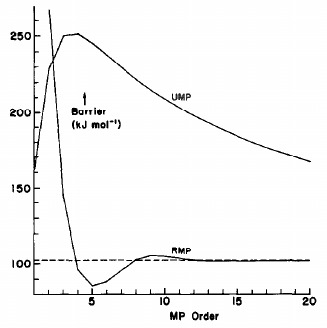
\includegraphics[width=\linewidth]{gill1986.png}
    \caption{Barriers to homolytic fission of \ce{He2^2+} at MPn/STO-3G level ($n = 1$--$20$) (taken from Ref.~\cite{Gill_1986}).}
    \label{fig:RUMP_Gill}
\end{wrapfigure}
When one relies on MP perturbation theory (and more generally on any perturbative partitioning), it would be reasonable to ask for a systematic improvement of the energy with respect to the perturbative order, i.e., one would expect that the more terms of the perturbative series one can compute, the closer the result from the exact energy.
%In other words, each time a higher-order term is computed, one would like to obtained an overall result closer to the exact energy. 
In other words, one would like a monotonic convergence of the MP series. Assuming this, the only limiting process to get the exact correlation energy (in a finite basis set) would be our ability to compute the terms of this perturbation series.
Unfortunately this is not as easy as one might think because i) the terms of the perturbative series become rapidly computationally cumbersome, and ii) erratic behavior of the perturbative coefficients are not uncommon. For example, in the late 80's, Gill and Radom reported deceptive and slow convergences in stretched systems \cite{Gill_1986, Gill_1988} (see also Refs.~\cite{Handy_1985, Lepetit_1988}). 
In Fig.~\ref{fig:RUMP_Gill}, which has been extracted from Ref.~\cite{Gill_1986}, one can see that the RMP series is convergent, yet oscillatory which is far from being convenient if one is only able to compute the first few terms of the expansion (for example here RMP5 is worse than RMP4). 
On the other hand, the UMP series is monotonically convergent (except for the first few orders) but very slowly. 
Thus, one cannot practically use it for systems where only the first terms can be computed.

When a bond is stretched, in most cases the exact wave function becomes more and more multi-reference. Yet the HF wave function is restricted to be a single Slater determinant.
Thus, it is inappropriate to model (even qualitatively) stretched systems. Nevertheless, the HF wave function can undergo a symmetry breaking to lower its energy by sacrificing one of the symmetry of the exact wave function during the process (see for example the case of \ce{H_2} in Ref.~\cite{SzaboBook}). 
One could then potentially claim that the RMP series exhibits deceptive convergence properties as the RHF Slater determinant is a poor approximation of the exact wave function for stretched system. However, even in the unrestricted formalism which clearly represents a better description of a stretched system, the UMP series does not have the smooth and rapidly converging behavior that one would wish for. 

\begin{table}
    \centering
    \caption{Percentage of electron correlation energy recovered and $\expval*{S^2}$ for the \ce{H2} molecule as a function of bond length (r,\si{\angstrom}) in the STO-3G basis set (taken from Ref.~\cite{Gill_1988}).}
    \begin{tabular}{ccccccc}
\hline
\hline
 $r$ & UHF & UMP2 & UMP3 & UMP4 & $\expval*{S^2}$ \\
\hline
0.75 & 0.0\% & 63.8\% & 87.4\% & 95.9\% & 0.00\\
1.35 & 0.0\% & 15.2\% & 26.1\% & 34.9\% & 0.49\\
2.00 & 0.0\% & 01.0\% & 01.8\% & 02.6\% & 0.95\\
2.50 & 0.0\% & 00.1\% & 00.3\% & 00.4\% & 0.99\\
\hline
\hline
\end{tabular}
    \label{tab:SpinContamination}
\end{table}

In the unrestricted framework the singlet ground state wave function is allowed to mix with triplet wave functions, leading to the so-called spin contamination issue. Gill \textit{et al.}~highlighted the link between slow convergence of the UMP series and spin contamination, as shown in Table \ref{tab:SpinContamination} for \ce{H2} in a minimal basis \cite{Gill_1988}. 
Handy and coworkers reported the same behavior of the series (oscillatory and slowly monotonically convergent) in stretched \ce{H2O} and \ce{NH2} systems \cite{Handy_1985}. Lepetit \textit{et al.}~analyzed the difference between the MP and EN partitioning for the UHF reference \cite{Lepetit_1988}. They concluded that the slow convergence is due to the coupling of the singly- and doubly-excited configurations. 
%Moreover, the MP and EN numerators in Eqs.~\eqref{eq:EMP2} and \eqref{eq:EEN2} are the same and they vanish when the bond length $r$ goes to infinity. Yet the MP denominators tends towards a constant when $r \to \infty$ so the terms vanish, whereas the EN denominators tends to zero which improves the convergence but can also make the series diverge.
Cremer and He analyzed 29 atomic and molecular systems at the FCI level \cite{Cremer_1996} and grouped them in two classes: i) the class A systems where one observes a monotonic convergence to the FCI energy, and ii) the class B for which convergence is erratic after initial oscillations. Their system set contains stretched molecules as well as molecules at their equilibrium geometry for various basis sets. They highlighted that \cite{Cremer_1996}
\begin{quote}
	\textit{``Class A systems are characterized by electronic structures with well-separated electron pairs while class B systems are characterized by electronic structures with electron clustering in one or more regions.''}
\end{quote}
As one can only compute the first terms of the MP series, a smart way of getting more accurate results is to use extrapolation formula, i.e., estimating the limit of the series with only few terms. 
Cremer and He proved that using specific extrapolation formulas of the MP series for class A and class B systems improves the precision of the results compared to the formula used without classes. The mean deviation from FCI correlation energies is $0.3$ millihartree with the adapted formula whereas with the formula that do not distinguish the systems it is 12 millihartree. 
Even if there were still shaded areas and that this classification was incomplete, this work showed that understanding the origin of the different modes of convergence would lead to a more rationalized use of the MP perturbation theory and to more accurate correlation energies.


\subsection{Cases of divergence}

In the late 90's, Olsen \textit{et al.}~discovered an even more preoccupying behavior of the MP series \cite{Olsen_1996}. They showed that the series could be divergent even in systems that they considered as well understood like \ce{Ne} and \ce{HF} (see Fig.~\ref{fig:NeHFDiv}) \cite{Olsen_1996, Christiansen_1996}. Cremer and He had already studied these two systems and classified them as ``class B'' systems. However, the analysis of Olsen and coworkers was performed in larger basis sets containing diffuse functions. In these basis sets, they found that the series become divergent at (very) high order.

\begin{figure}
    \centering
    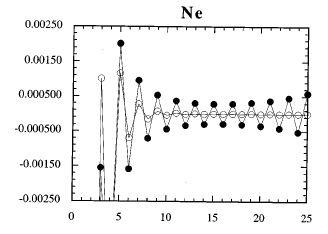
\includegraphics[width=0.45\textwidth]{Nedivergence.png}
    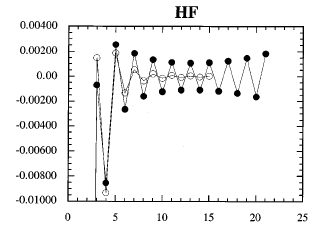
\includegraphics[width=0.45\textwidth]{HFdivergence.png}
    \caption{\centering Correlation contributions for \ce{Ne} and \ce{HF} in the cc-pVTZ-(f/d) $\circ$ and aug-cc-pVDZ $\bullet$ basis sets (taken from Ref.~\cite{Olsen_1996}).}
    \label{fig:NeHFDiv}
\end{figure}

The discovery of this divergent behavior is worrying as in order to get meaningful and accurate energies, calculations must be performed in large basis sets (as close as possible from the complete basis set limit). Including diffuse functions is particularly important in the case of anions and/or Rydberg excited states where the wave function is much more diffuse than the ground-state one. As a consequence, they investigated further the causes of these divergences as well as the reasons of the different types of convergence. To do so, they analyzed the relation between the dominant singularity (i.e., the closest singularity to the origin) and the convergence behavior of the series \cite{Olsen_2000}. Their analysis is based on Darboux's theorem: 
\begin{quote}
	\textit{``In the limit of large order, the series coefficients become equivalent to the Taylor series coefficients of the singularity closest to the origin. Following the result of this theorem, the convergence patterns of the MP series can be explained by looking at the dominant singularity.''}
\end{quote}

A singularity in the unit circle is designated as an intruder state, more precisely as a front-door (respectively back-door) intruder state if the real part of the singularity is positive (respectively negative). Their method consists in performing a scan of the real axis to detect the avoided crossing responsible for the pair of dominant singularities. Then by modeling this avoided crossing via a two-state Hamiltonian one can get an approximation of the dominant conjugate pair of singularities by finding the EPs of the following $2\times2$ Hamiltonian
\begin{equation}
\underbrace{\mqty(\alpha & \delta \\ \delta & \beta)}_{\hH} = \underbrace{\mqty(\alpha + \alpha_s & 0 \\ 0 & \beta + \beta_s )}_{\hH^{(0)}} + \underbrace{\mqty(- \alpha_s & \delta \\ \delta & - \beta_s)}_{\hV},
\end{equation}
where the diagonal matrix is the unperturbed Hamiltonian and the other matrix is the perturbation.

They first studied molecules with low-lying doubly-excited states of the same spatial and spin symmetry.
% \titou{because in those systems the HF wave function is a bad approximation.} 
The exact wave function has a non-negligible contribution from the doubly-excited states, so these low-lying excited states were good candidates for being intruder states. For \ce{CH_2} in a large basis set, the series is convergent up to the 50th order. They showed that the dominant singularity lies outside the unit circle but close to it causing the slow convergence.

Then they demonstrated that the divergence for \ce{Ne} is due to a back-door intruder state. When the basis set is augmented with diffuse functions, the ground state undergo sharp avoided crossings with highly diffuse excited states leading to a back-door intruder state. They used their two-state model on this avoided crossings and the model was actually predicting the divergence of the series. 
%They concluded that the divergence of the series was due to the interaction with a highly diffuse excited state. 

Moreover they proved that the extrapolation formulas of Cremer and He \cite{Cremer_1996} cannot be used for all systems, and that these formulas were not mathematically motivated when looking at the singularity causing the divergence. For example, the hydrogen fluoride molecule contains both back-door intruder states and low-lying doubly-excited states which results in alternated terms up to 10th order. For higher orders, the series is monotonically convergent. This surprising behavior is due to the fact that two pairs of singularities are approximately at the same distance from the origin.

\subsection{The singularity structure}

In the 2000's, Sergeev and Goodson \cite{Sergeev_2005, Sergeev_2006} analyzed this problem from a more mathematical point of view by looking at the whole singularity structure where Olsen and collaborators were trying to find the dominant singularity causing the divergence. They regrouped singularities in two classes: i) $\alpha$ singularities which have ``large'' imaginary parts, and ii) $\beta$ singularities which have very small imaginary parts. Singularities of type $\alpha$ are related to large avoided crossing between the ground and low-lying excited states, whereas $\beta$ singularities come from a sharp avoided crossing between the ground state and a highly diffuse state. They succeeded to explain the divergence of the series caused by $\beta$ singularities following previous work of Stillinger \cite{Stillinger_2000}. 

To understand the convergence properties of the perturbation series at $\lambda=1$, one must look at the whole complex plane, in particular, for negative (i.e., real) values of $\lambda$. If $\lambda$ is negative, the Coulomb interaction becomes attractive but the mean field (which has been computed at $\lambda = 1$) remains repulsive as it is proportional to $(1-\lambda)$:

\begin{equation}\label{eq:HamiltonianStillinger}
    \hH(\lambda) = 
    \sum_{i}^{n} \qty[ 
    \underbrace{-\frac{1}{2}\grad_i^2 
    - \sum_{A}^{N} \frac{Z_A}{\abs{\vb{r}_i-\vb{R}_A}}}_{\text{Independent of $\lambda$}}
    + \overbrace{(1-\lambda)v^{\text{HF}}(\vb{x}_i)}^{\textcolor{red}{\text{Repulsive for $\lambda < 1$}}}
    + \underbrace{\lambda\sum_{i<j}^{n}\frac{1}{|\vb{r}_i-\vb{r}_j|}}_{\textcolor{blue}{\text{Attractive for $\lambda < 0$}}} 
    ].
\end{equation}

The major difference between those two terms is that the repulsive mean field is localized around the nuclei whereas the interelectronic interaction persist away from the nuclei. If $\lambda$ becomes more and more negative the mean field becomes more and more repulsive so there exists a critical (negative) value of $\lambda$, $\lambda_\text{c}$, for which the Coulombic field created by the nuclei cannot bind the electrons anymore because of the $\lambda$-independent nature of the the electron-nucleus attraction. For $\lambda = \lambda_c$, the electrons dissociate from the nuclei and form a bound cluster which is infinitely separated from the nuclei. According to Baker \cite{Baker_1971}, this value is a critical point of the system and, by analogy with thermodynamics, the energy $E(\lambda)$ exhibits a singularity at $\lambda_\text{c}$. At this point the system undergo a phase transition and a symmetry breaking. Beyond $\lambda_c$ there is a continuum of eigenstates with electrons dissociated from the nucleus.

This reasoning is done on the exact Hamiltonian and energy, i.e., the Hamiltonian in the complete Hilbert space, this is the exact energy which exhibits this singularity on the negative real axis. However, in a finite basis set which does not span the complete Hilbert space, one can prove that, for a Hermitian Hamiltonian, the singularities of $E(\lambda)$ occurs in complex conjugate pairs with non-zero imaginary parts. Sergeev and Goodson proved \cite{Sergeev_2005}, as predicted by Stillinger \cite{Stillinger_2000}, that in a finite basis set the critical point on the real axis is modeled by a cluster of sharp avoided crossings with diffuse functions, equivalently by a cluster of $\beta$ singularities in the negative half plane. This explains that Olsen \textit{et al.}, because they used a simple $2\times2$ model, only observed the first singularity of this cluster of singularities causing the divergence.

Finally, it was shown that $\beta$ singularities are very sensitive to changes in the basis set but not to the stretching of the system. On the contrary $\alpha$ singularities are relatively insensitive to the basis sets but very sensitive to bond stretching. According to Goodson \cite{Goodson_2004}, the singularity structure of stretched molecules is difficult because there is more than one significant singularity. This is consistent with the observation of Olsen and coworkers \cite{Olsen_2000} on the \ce{HF} molecule at equilibrium geometry and stretched geometry. To the best our knowledge, the effect of bond stretching on singularities, its link with spin contamination and symmetry breaking of the wave function has not been as well understood as the ionization phenomenon and its link with diffuse functions.  In this work, we shall try to improve our understanding of the effect of symmetry breaking on the singularities of $E(\lambda)$ and we hope that it will lead to a deeper understanding of perturbation theory.

\subsection{The physics of quantum phase transition}

In the previous section, we saw that a careful analysis of the structure of the Hamiltonian allows us to predict the existence of a critical point. In a finite basis set this critical point is model by a cluster of $\beta$ singularities. It is now well known that this phenomenon is a special case of a more general phenomenon. Indeed, theoretical physicists proved that EPs close to the real axis are connected to \textit{quantum phase transitions} (QPTs) \cite{Heiss_1988, Heiss_2002, Cejnar_2005, Cejnar_2007, Cejnar_2009, Borisov_2015, Sindelka_2017}. In quantum mechanics, the Hamiltonian is almost always dependent of, at least, one parameter. In some cases the variation of a parameter can lead to abrupt changes at a critical point. These QPTs exist both for ground and excited states as shown by Cejnar and coworkers \cite{Cejnar_2009, Sachdev_2011, Cejnar_2015, Cejnar_2016, Caprio_2008, Macek_2019}. A ground-state QPT is characterized by the derivatives of the ground-state energy with respect to a non-thermal control parameter \cite{Cejnar_2009, Sachdev_2011}. The transition is called discontinuous and of first order if the first derivative is discontinuous at the critical parameter value. Otherwise, it is called continuous and of $m$th order if the $m$th derivative is discontinuous. A QPT can also be identify by the discontinuity of an appropriate order parameter (or one of its derivatives). 

The presence of an EP close to the real axis is characteristic of a sharp avoided crossing. Yet, at such an avoided crossing, eigenstates change abruptly. Although it is now well understood that EPs are closely related to QPTs, the link between the type of QPT (ground state or excited state, first or higher order) and EPs still need to be clarified. One of the major obstacles that one faces in order to achieve this resides in the ability to compute the distribution of EPs. The numerical assignment of an EP to two energies on the real axis is very difficult in large dimensions. Hence, the design of specific methods are required to get information on the location of EPs. Following this idea, Cejnar \textit{et al.}~developed a method based on a Coulomb analogy giving access to the density of EP close to the real axis \cite{Cejnar_2005, Cejnar_2007}. More recently Stransky and coworkers proved that the distribution of EPs is characteristic on the order of the QPT \cite{Stransky_2018}. In the thermodynamic limit, some of the EPs converge towards a critical point $\lambda^\text{c}$ on the real axis. They showed that, within the interaction boson model \cite{Lipkin_1965}, EPs associated to first- and second-order QPT behave differently when the number of particles increases. The position of these singularities converge towards the critical point on the real axis at different rates (exponentially and algebraically for the first and second order, respectively) with respect to the number of particles.

It seems like our understanding of the physics of spatial and/or spin symmetry breaking in HF theory can be enlightened by QPT theory. Indeed, the second derivative of the HF ground-state energy is discontinuous at the point of spin symmetry-breaking which means that the system undergo a second-order QPT. Moreover, the $\beta$ singularities introduced by Sergeev and coworkers to describe the EPs modeling the formation of a bound cluster of electrons are actually a more general class of singularities. The EPs close to the real axis (the so-called $\beta$ singularities) are connected to QPT because they result from a sharp avoided crossings at which the eigenstates change quickly. However, the $\alpha$ singularities arise from large avoided crossings. Thus, they cannot be connected to QPT. The avoided crossings generating $\alpha$ singularities generally involve the ground state and low-lying doubly-excited states. Those excited states have a non-negligible contribution to the exact FCI solution because they have the same spatial and spin symmetry as the ground state. We believe that $\alpha$ singularities are connected to states with non-negligible contribution in the CI expansion thus to the dynamical part of the correlation energy, while $\beta$ singularities are linked to symmetry breaking and phase transitions of the wave function, i.e., to the multi-reference nature of the wave function thus to the static part of the correlation energy.


%============================================================%
\section{The spherium model}\label{sec:spherium}
%============================================================%

Simple systems that are analytically solvable (or at least quasi-exactly solvable, i.e., models for which it is possible to obtain a finite portion of the exact solutions of the Schr{\"o}dinger equation \cite{Ushveridze_1994}) are of great importance in theoretical chemistry. 
These systems are very useful to perform benchmark studies in order to test new methods as the mathematics are easier than in realistic systems (such as molecules or solids) but retain much of the key physics. 
To investigate the physics of EPs we consider one such system named \textit{spherium}. 
It consists of two electrons confined to the surface of a sphere interacting through the long-range Coulomb potential \cite{Thompson_2005, Seidl_2007, Loos_2009b}. 
Thus, the Hamiltonian is
\begin{equation}
	\hH = -\frac{\grad_1^2 + \grad_2^2}{2} + \frac{1}{r_{12}},
\end{equation}
or
\begin{equation} \label{eq:H-sph-omega}
	\hH = -\frac{1}{R^2} \qty( \pdv[2]{}{\omega} + \cot \omega \pdv{}{\omega}) + \frac{1}{R \sqrt{2 - 2 \cos \omega}},
\end{equation}
where $\omega$ is the interelectronic angle.
The Laplace operators are the kinetic operators for each electrons and $r_{12}^{-1} = \abs{\vb{r}_1 - \vb{r}_2}^{-1}$ is the Coulomb operator. 
Note that, as readily seen by the definition of the interelectronic distance $r_{12}$, the electrons interact through the sphere.
The radius of the sphere $R$ dictates the correlation regime \cite{Loos_2009}. 
In the weak correlation regime (i.e., small $R$), the kinetic energy (which scales as $R^{-2}$) dominates and the electrons are delocalized over the sphere.
For large $R$ (or strong correlation regime), the electron repulsion term (which scales as $R^{-1}$) drives the physics and the electrons localize on opposite side of the sphere to minimize their Coulomb repulsion. 
This phenomenon is sometimes referred to as a Wigner crystallization \cite{Wigner_1934}.

We will use this model in order to rationalize the effects of the parameters that may influence the physics of EPs:
\begin{itemize}
	\item Partitioning of the Hamiltonian and the actual zeroth-order reference: weak correlation reference (RHF or UHF references, MP or EN partitioning), or strongly correlated reference.
	\item Basis set: minimal basis or infinite (i.e., complete) basis.
	\item Radius of the sphere that ultimately dictates the correlation regime.
\end{itemize}

In the RHF formalism, the two electrons are restricted to ``live'' in the same spatial orbital.
The spatial part of the RHF wave function is then
\begin{equation}\label{eq:RHF_WF}
	\Psi_{\text{RHF}}(\theta_1,\theta_2) = Y_0(\theta_1) Y_0(\theta_2),
\end{equation}
where $\theta_i$ is the polar angle of the $i$th electron and $Y_{\ell}(\theta)$ is a zonal spherical harmonic. 
Because $Y_0(\theta) = 1/\sqrt{4\pi}$, it is clear that the RHF wave function yields a uniform one-electron density.

The RHF wave function cannot model properly the physics of the system at large $R$ because the spatial orbitals are restricted to be the same, and, \textit{a fortiori}, it cannot represent two electrons on opposite side of the sphere. 
Within the UHF formalism, there is a critical value of $R$, called Coulson-Fischer point \cite{Coulson_1949}, at which a UHF solution appears and is lower in energy than the RHF one.
The UHF solution has broken symmetry because the two electrons tends to localize on opposite sides of the sphere. 
The spatial part of the UHF wave function is defined as
\begin{equation}\label{eq:UHF_WF}
	\Psi_{\text{UHF}}(\theta_1,\theta_2)=\phi_\alpha(\theta_1)\phi_\beta(\theta_2),
\end{equation}
where $\phi_\sigma(\theta)$ is the spatial orbital associated with the spin-$\sigma$ electrons ($\sigma = \alpha$ for spin-up electrons and $\sigma = \beta$ for spin-down electrons).
These one-electron orbitals are expanded in the basis of zonal spherical harmonics
\begin{equation}
	\phi_\sigma(\theta)=\sum_{\ell=0}^{\infty}C_{\sigma,\ell}Y_{\ell}(\theta)
\end{equation}
It is possible to obtain the formula for the HF energy in this basis set \cite{Loos_2009}:
\begin{equation}
	E_{\text{HF}} = T_{\text{HF}} + V_{\text{HF}},
\label{eq:EHF}
\end{equation}
where the kinetic and potential energies are, respectively,
\begin{align}
	T_{\text{HF}} & = \frac{1}{R^2} \sum_{\sigma=\alpha,\beta} \sum_{\ell=0}^{\infty} C_{\sigma,\ell}^2 \, \ell(\ell+1),
	&
	V_{\text{HF}} & = \frac{1}{R} \sum_{L=0}^{\infty}
	v^\alpha_{L} v^\beta_{L},
\end{align}
and
\begin{equation}
	v^\sigma_{L} 
	=  \sum_{\ell_1,\ell_2} \sqrt{(2\ell_1+1)(2\ell_2+1)} C_{\sigma,\ell_1}C_{\sigma,\ell_2}
	\begin{pmatrix}
		\ell_1 & \ell_2 & L 
		\\
		0 & 0 & 0
	\end{pmatrix}^2 
\end{equation}
is expressed in terms of the Wigner 3j-symbols \cite{AngularBook}.

The general method is to use a self-consistent field procedure as described in Ref.~\cite{SzaboBook} to get the coefficients of the HF wave function corresponding to stationary solutions with respect to the coefficients $C_{\sigma,\ell}$, i.e.,
\begin{equation}
	\pdv{E_{\text{HF}}}{C_{\sigma,\ell}} = 0.
\end{equation}
Here, we work in a minimal basis, composed of $Y_{0}$ and $Y_{1}$, or equivalently, a s and p\textsubscript{z} orbital, to illustrate the difference between the RHF and UHF solutions. In this basis there is a shortcut to find the stationary solutions and ensure normalization of the orbitals. One can define the one-electron orbitals as
\begin{equation}
	\phi_\sigma(\theta)= \cos(\chi_\sigma)Y_{0}(\theta) + \sin(\chi_\sigma)Y_{1}(\theta),
\end{equation}
using a mixing angle between the two basis functions for each spin manifold. 
Hence, one has just to minimize/maximize the energy with respect to the two mixing angles $\chi_\alpha$ and $\chi_\beta$.
 
This process provides the three following solutions valid for all value of $R$, which are respectively a minimum, a maximum and a saddle point of the HF equations:
\begin{itemize}
\item The two electrons are in the s orbital which is a RHF solution. This solution is associated with the energy $1/R$.
\item The two electrons are in the p\textsubscript{z} orbital which is a RHF solution. This solution is associated with the energy $2/R^{2}+ 29/(25R)$.
\item One electron is in the s orbital and the other is in the p\textsubscript{z} orbital which is a UHF solution. This solution is associated with the energy $1/R^{2} + 1/R$.
\end{itemize}

In addition, the minimization process gives also the well-known symmetry-broken UHF (sb-UHF) solution. In this case the Coulson-Fischer point associated to this solution is $R=3/2$. For $R>3/2$ the sb-UHF solution is the global minimum of the HF equations and the RHF solution presented before is a local minimum. This solution corresponds to the configuration with the spin-up electron in an orbital on one side of the sphere and the spin-down electron in a miror-image orbital on the opposite side and the configuration the other way round. The electrons can be on opposite sides of the sphere because the choice of p\textsubscript{z} as a basis function induced a privileged axis on the sphere for the electrons. For $R>3/2$, this solution has the energy
\begin{equation}\label{eq:EsbUHF}
	E_{\text{sb-UHF}}=-\frac{75}{112R^3}+\frac{25}{28R^2}+\frac{59}{84R}.
\end{equation}

The exact solution for the ground state is a singlet. The spherical harmonics are eigenvectors of $\hS^2$ (the spin operator) and they are associated to different eigenvalues. Yet, the symmetry-broken orbitals are linear combinations of $Y_0$ and $Y_1$. Hence, the symmetry-broken orbitals are not eigenvectors of $\hS^2$. However, this solution gives lower energies than the RHF one at large $R$ as shown in Table \ref{tab:ERHFvsEUHF} even if it does not have the exact spin symmetry. In fact, at the Coulson-Fischer point, it becomes more effective to minimize the Coulomb repulsion than the kinetic energy in order to minimize the total energy. Thus, within the HF approximation, the variational principle is allowed to break the spin symmetry because it yields a more effective minimization of the Coulomb repulsion. This type of symmetry breaking is called a spin density wave because the system oscillates between the two symmetry-broken configurations \cite{GiulianiBook}.

\begin{table}
\centering
\caption{RHF and sb-UHF energies in the minimal basis and exact energies (in the complete basis) for various $R$.}
\begin{tabular}{ccccccccc}
\hline
\hline
$R$ & 0.1 & 1 & 2 & 3 & 5 & 10 & 100 & 1000 \\
\hline
RHF 	& 10.00000 & 1.000000 & 0.500000 & 0.333333 & 0.200000 & 0.100000 & 0.010000 & 0.001000 \\
UHF 	& 10.00000 & 1.000000 & 0.490699 & 0.308532 & 0.170833 & 0.078497 & 0.007112 & 0.000703 \\
Exact 	& 9.783874 & 0.852781 & 0.391959 & 0.247898 & 0.139471 & 0.064525 & 0.005487 & 0.000515 \\
\hline
\hline
\end{tabular}
\label{tab:ERHFvsEUHF}
\end{table}

There is also another symmetry-broken solution for $R>75/38$ but this one corresponds to a maximum of the HF equations. This solution is associated with another type of symmetry breaking somewhat less known. It corresponds to a configuration where both electrons are on the same side of the sphere, in the same spatial orbital. This solution is called symmetry-broken RHF (sb-RHF). \antoine{The reasoning is counter-intuitive because the electrons tends to maximize their energy. If the orbitals are symmetric, the maximum is when the two electrons are in the p\textsubscript{z} orbital because it maximizes the kinetic energy. At the critical value of $R$, placing the two electrons in the same symmetry-broken orbital i.e., on the same side of the sphere gives a superior energy than the p\textsubscript{z}\textsuperscript{2} state. This is because it becomes more efficient to maximize the repulsion energy than the kinetic energy for $R>75/38$.}
This configuration breaks the spatial symmetry of charge. Hence this symmetry breaking is associated with a charge density wave, the system oscillates between the situations with the two electrons on each side \cite{GiulianiBook}.
The energy associated with this sb-RHF solution reads
\begin{equation}
E_{\text{sb-RHF}}=\frac{75}{88R^3}+\frac{25}{22R^2}+\frac{91}{66R}.
\end{equation}

\begin{figure}[h!]
    \centering
    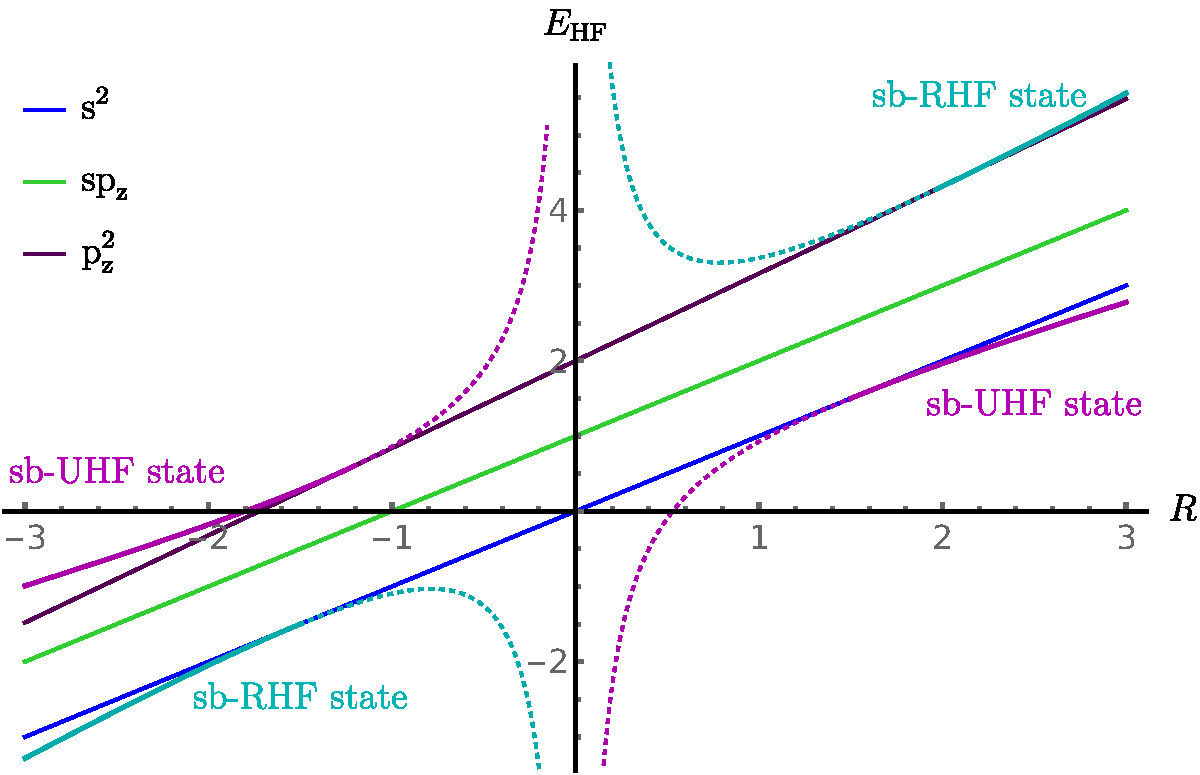
\includegraphics[width=0.8\linewidth]{EsbHF.pdf}
    \caption{Energies of the five solutions of the HF equations (multiplied by $R^2$). The dotted curves correspond to the analytic continuation of the symmetry-broken solutions.}
    \label{fig:SpheriumNrj}
\end{figure}

We can also consider negative values of $R$, which corresponds to the situation where one of the electrons is replaced by a positron (the anti-particle of the electron) as readily seen in Eq.~\eqref{eq:H-sph-omega}. For negative $R$ values, there are also a sb-RHF ($R<-3/2$) and a sb-UHF ($R<-75/38$) solution for negative values of $R$ (see Fig.~\ref{fig:SpheriumNrj}) but in this case the sb-RHF solution is a minimum and the sb-UHF is a maximum of the HF equations. Indeed, the sb-RHF state minimizes the attraction energy by placing the electron and the positron on the same side of the sphere. And the sb-UHF state maximizes the energy because the two attracting particles are on opposite sides of the sphere.

In addition, we can also consider the symmetry-broken solutions beyond their respective Coulson-Fischer points by analytically continuing their respective energies leading to the so-called holomorphic solutions \cite{Hiscock_2014, Burton_2019, Burton_2019a}. All those energies are plotted in Fig.~\ref{fig:SpheriumNrj}. The dotted curves corresponds to the holomorphic domain of the energies.


\section{Radius of convergence and exceptional points}

\subsection{Evolution of the radius of convergence}

In this subsection, we investigate how the partitioning of $\hH(\lambda)$ influence the radius of convergence of the perturbation series. Let us remind the reader that the radius of convergence is equal to the distance of the closest singularity to the origin of $E(\lambda)$. Hence, we have to determine the locations of the EPs to obtain information on the convergence properties of the perturbative series. To find them we solve simultaneously the following equations \cite{Cejnar_2007}:
\begin{subequations}
\begin{align}
	\label{eq:PolChar}
	\det[E\hI-\hH(\lambda)] & = 0,
	\\ 
	\label{eq:DPolChar}
	\pdv{E}\det[E\hI-\hH(\lambda)] & = 0,
\end{align}
\end{subequations}
where $\hI$ is the identity operator.
Equation \eqref{eq:PolChar} is the well-known secular equation providing us with the (eigen)energies of the system. If an energy is also solution of Eq.~\eqref{eq:DPolChar}, then this energy is, at least two-fold degenerate. In this case the energies obtained are dependent of $\lambda$. Thus, solving these equations with respect to $E$ and $\lambda$ gives the value of $\lambda$ where two energies are degenerate. These degeneracies can be conical intersections between two states with different symmetry for real values of $\lambda$ \cite{Yarkony_1996} or EPs between two states with the same symmetry for complex values of $\lambda$.

Let us assume that electron 1 is spin-up and electron 2 is spin-down. 
Hence, we can forget about the spin part of the spin-orbitals and from now on we will work with spatial orbitals. In the restricted formalism the spatial orbitals are the same so the two-electron basis set can be defined as

\begin{align}\label{eq:rhfbasis}
 \psi_1 & =Y_{0}(\theta_1)Y_{0}(\theta_2),
 & 
 \psi_2 & =Y_{0}(\theta_1)Y_{1}(\theta_2),\\
 \psi_3 & =Y_{1}(\theta_1)Y_{0}(\theta_2),
 & 
 \psi_4 & =Y_{1}(\theta_1)Y_{1}(\theta_2).
\end{align}
The Hamiltonian $\hH(\lambda)$ is block diagonal in this basis because of its symmetry, i.e., $\psi_1$ only interacts with $\psi_4$, and $\psi_2$ with $\psi_3$. The two singly-excited states yield, after diagonalization, a spatially anti-symmetric singlet sp\textsubscript{z} and a spatially symmetric triplet sp\textsubscript{z} state. Hence those states do not have the same symmetry as the spatially symmetric singlet ground state. Thus, these states cannot be involved in an avoided crossing with the ground state as can be seen in Fig.~\ref{fig:RHFMiniBas} and, \textit{a fortiori} cannot be involved in an EP with the ground state. However there is an avoided crossing between the s\textsuperscript{2} and p\textsubscript{z}\textsuperscript{2} states which gives two EPs in the complex plane. 

\begin{wrapfigure}{R}{0.5\textwidth}
    \centering
    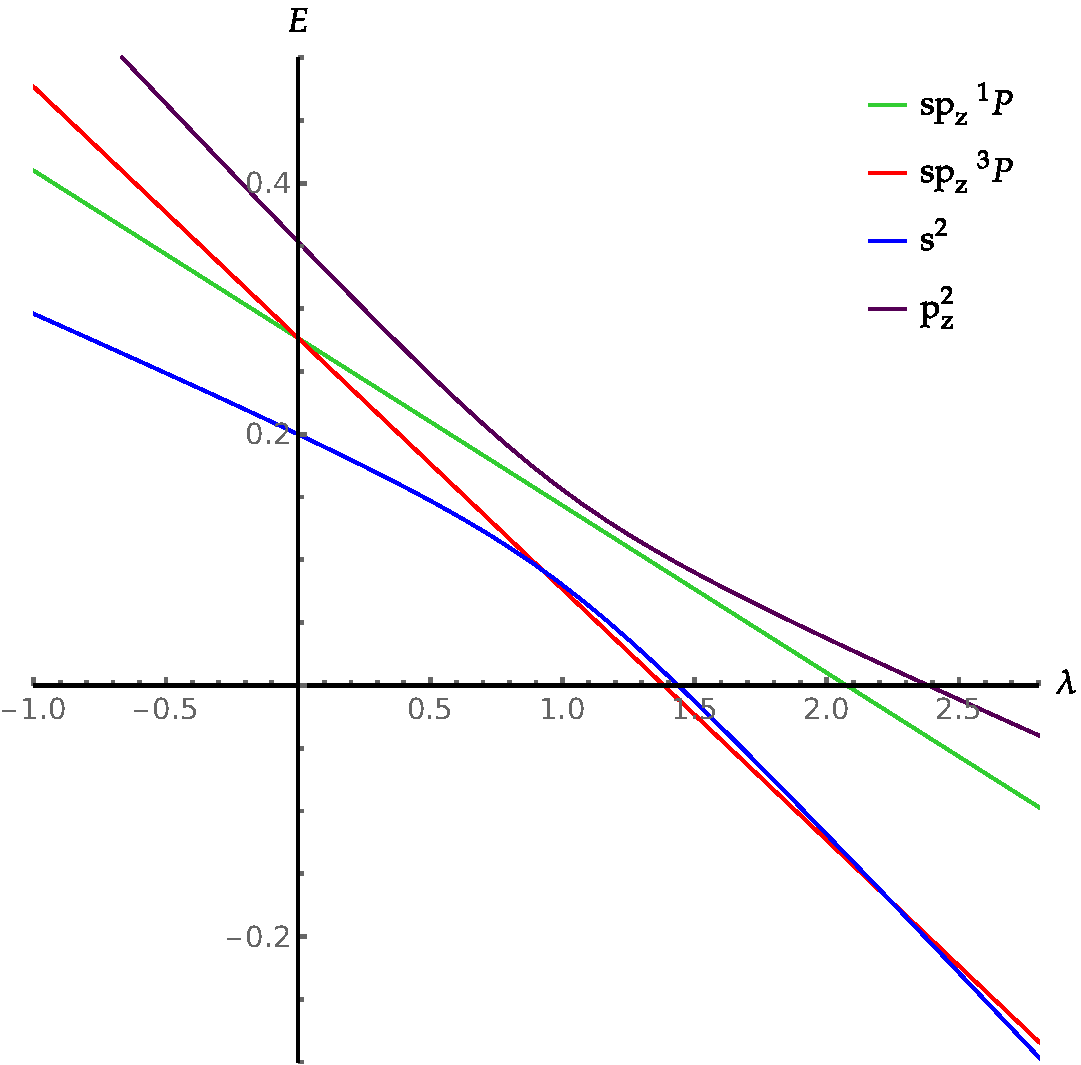
\includegraphics[width=\linewidth]{EMP_RHF_R10.pdf}
    \caption{Energies $E(\lambda)$ in the restricted basis set \eqref{eq:rhfbasis} with $R=10$.
    One can clearly see the avoided crossing between the s\textsuperscript{2} and p\textsubscript{z}\textsuperscript{2} states around $\lambda = 1$.}
    \label{fig:RHFMiniBas}
\end{wrapfigure}

To simplify the problem, it is convenient to only consider basis functions of a given symmetry. Such basis functions are called configuration state functions (CSFs). It simplifies greatly the problem because, with such a basis set, one only gets the degeneracies of interest associated with the convergence properties, i.e., the EPs between states with the same symmetry as the ground state. In the present context, the ground state is a totally symmetric singlet. According to angular momentum theory \cite{AngularBook, SlaterBook, Loos_2009}, we expand the exact wave function in the following two-electron basis:
\begin{equation}
\Phi_\ell(\omega)=\frac{\sqrt{2\ell+1}}{4\pi R^2}P_\ell(\cos\omega),
\end{equation}
where $P_\ell$ are Legendre polynomials.

Then, using this basis set we can compare the different partitioning of Sec.~\ref{sec:AlterPart}. Figure \ref{fig:RadiusPartitioning} shows the evolution of the radius of convergence $R_{\text{CV}}$ as a function of $R$ for the MP, the EN, the WC and the SC partitioning in a minimal basis (i.e., consisting of $P_0$ and $P_1$) of size $K = 2$, and in the same basis augmented with $P_2$ ($K = 3$). We see that, for the SC partitioning, $R_{\text{CV}}$ increases with $R$ whereas it is decreasing for the three others partitioning. This result is expected because the MP, EN, and WC partitioning use a weakly correlated reference so $\hH^{(0)}$ is a good approximation for small $R$. On the contrary, the SC partitioning consider naturally a strongly correlated reference so the SC series converges far better when the electron are strongly correlated, i.e., when $R$ is large in the spherium model.

Interestingly, the radius of convergence associated with the SC partitioning is greater than one for a greater range of radii for $K = 2$ than $K = 3$. 
In the complete basis limit, the radius of convergence of the SC partitioning is greater than unity only for very large value of $R$.
The MP partitioning is always better than WC in Fig.~\ref{fig:RadiusPartitioning}. In the WC partitioning the powers of $R$ (the zeroth-order scales as $R^{-2}$ while the perturbation scales as $R^{-1}$) are well-separated so each term of the series has a well-defined power of $R$. This is not the case for the MP series.
Interestingly, it can be proved that the $m$th order energy of the WC series can be obtained as a Taylor series of MP$m$ with respect to $R$. 
It seems that the EN is better than MP for very small $R$ in the minimal basis. In fact, it is just an artefact of the minimal basis because, for $K = 3$, the MP series has a greater radius of convergence for all values of $R$ \antoine{and this is still true for $K>3$.}

\begin{figure}
    \centering
    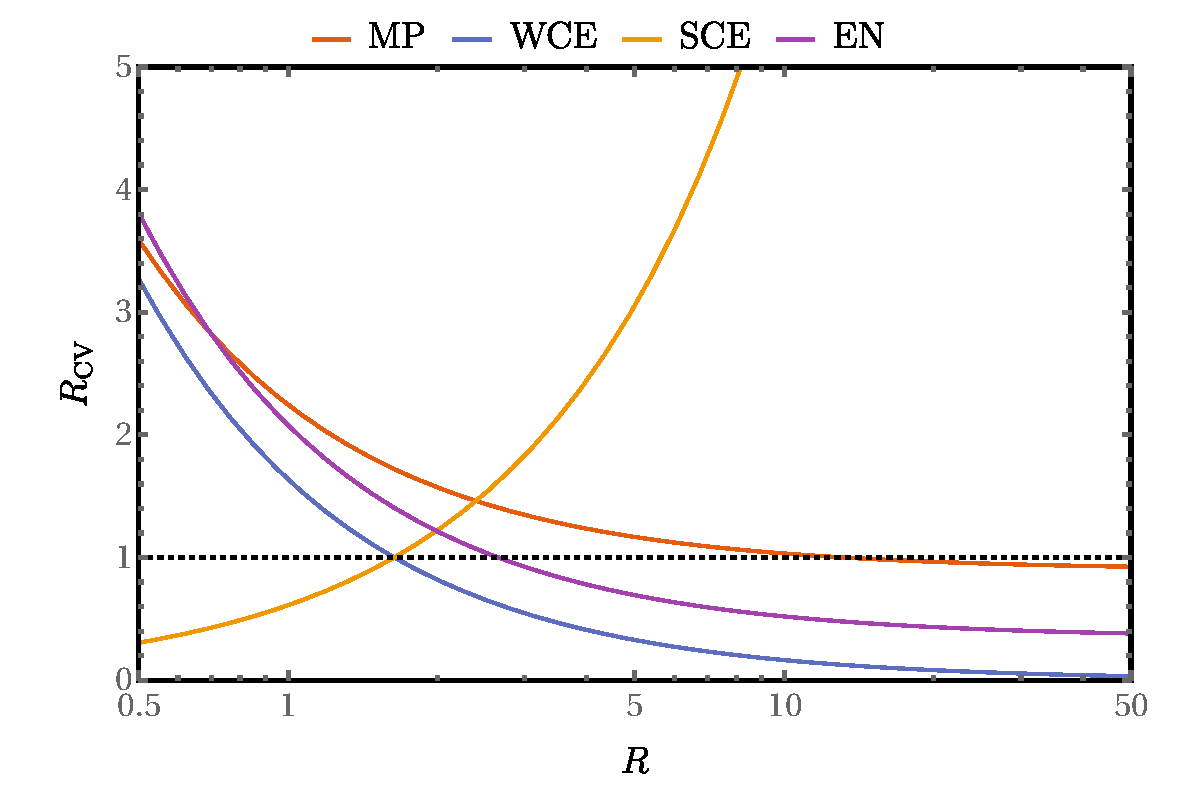
\includegraphics[width=0.49\textwidth]{PartitioningRCV2.pdf}
    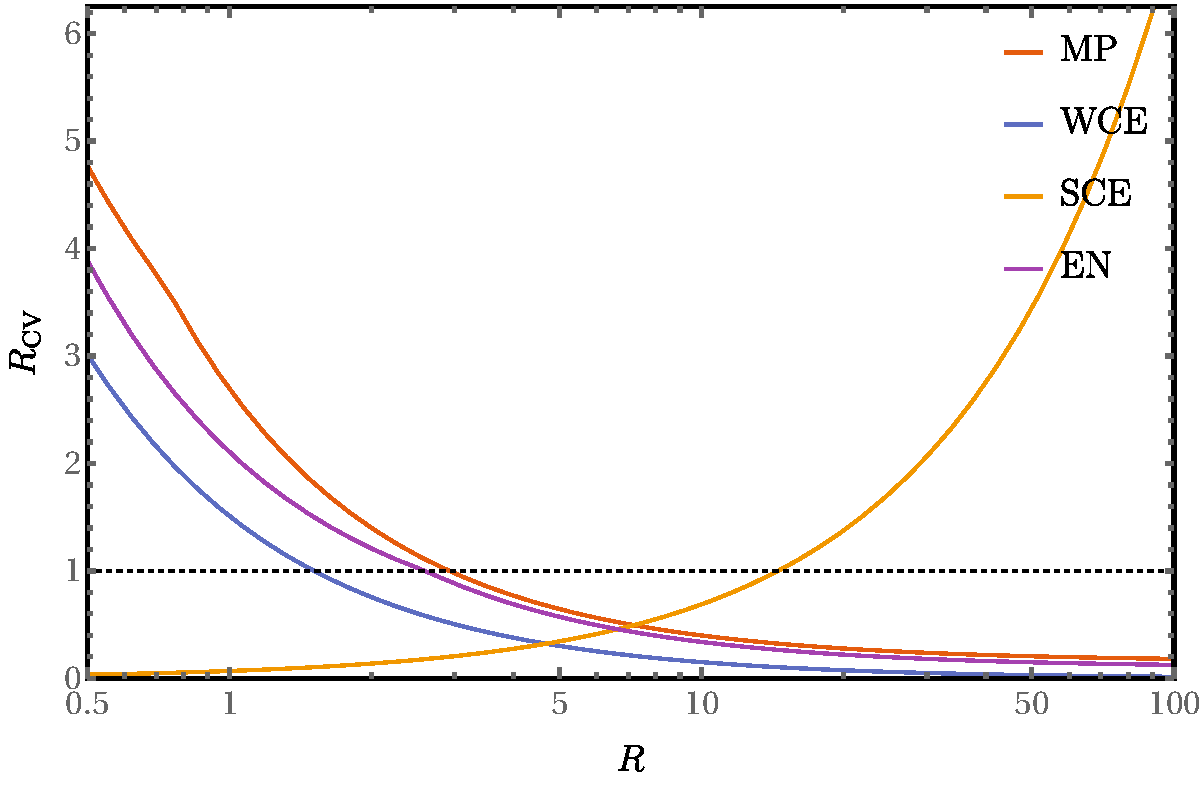
\includegraphics[width=0.49\textwidth]{PartitioningRCV3.pdf}
    \caption{Radius of convergence $R_{\text{CV}}$ for two (left) and three (right) basis functions for various partitionings.}
    \label{fig:RadiusPartitioning}
\end{figure}

The MP partitioning is always better than WC in Fig.~\ref{fig:RadiusPartitioning}. In the WC partitioning the powers of $R$ (the zeroth-order scales as $R^{-2}$ while the perturbation scales as $R^{-1}$) are well-separated so each term of the series has a well-defined power of $R$. This is not the case for the MP series.
Interestingly, it can be proved that the $m$th order energy of the WC series can be obtained as a Taylor series of MP$m$ with respect to $R$. 
It seems that the EN is better than MP for very small $R$ in the minimal basis. In fact, it is just an artefact of the minimal basis because, for $K = 3$, the MP series has a greater radius of convergence for all values of $R$. It holds true for $K>3$.


Figure \ref{fig:RadiusBasis} shows that the radius of convergence is not very sensitive to the size of the basis set. The CSFs have all the same spin and spatial symmetries so we expect that the singularities obtained within this basis set will be $\alpha$ singularities. Table \ref{tab:SingAlpha} shows that the singularities considered in this case are indeed $\alpha$ singularities. This is consistent with the observation of Goodson and Sergeev \cite{Goodson_2004} who stated that $\alpha$ singularities are relatively insensitive to the basis set size. The discontinuities observed in Fig.~\ref{fig:RadiusBasis} for the MP partitioning are due to changes in dominant singularity. We can observe this change in Table \ref{tab:SingAlpha}, the value for $R=1$ and $R=2$ are respectively in the positive and negative planes.

\begin{figure}[h!]
    \centering
    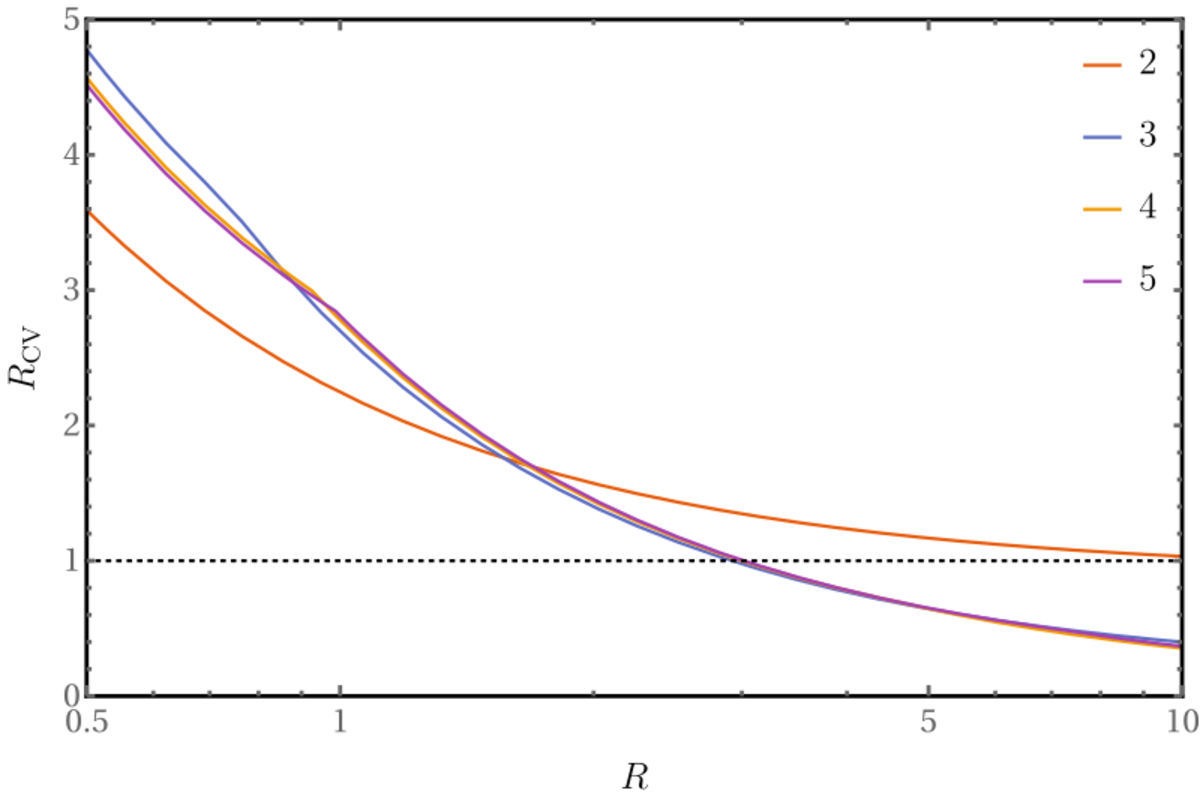
\includegraphics[width=0.49\textwidth]{MPlargebasis.pdf}
    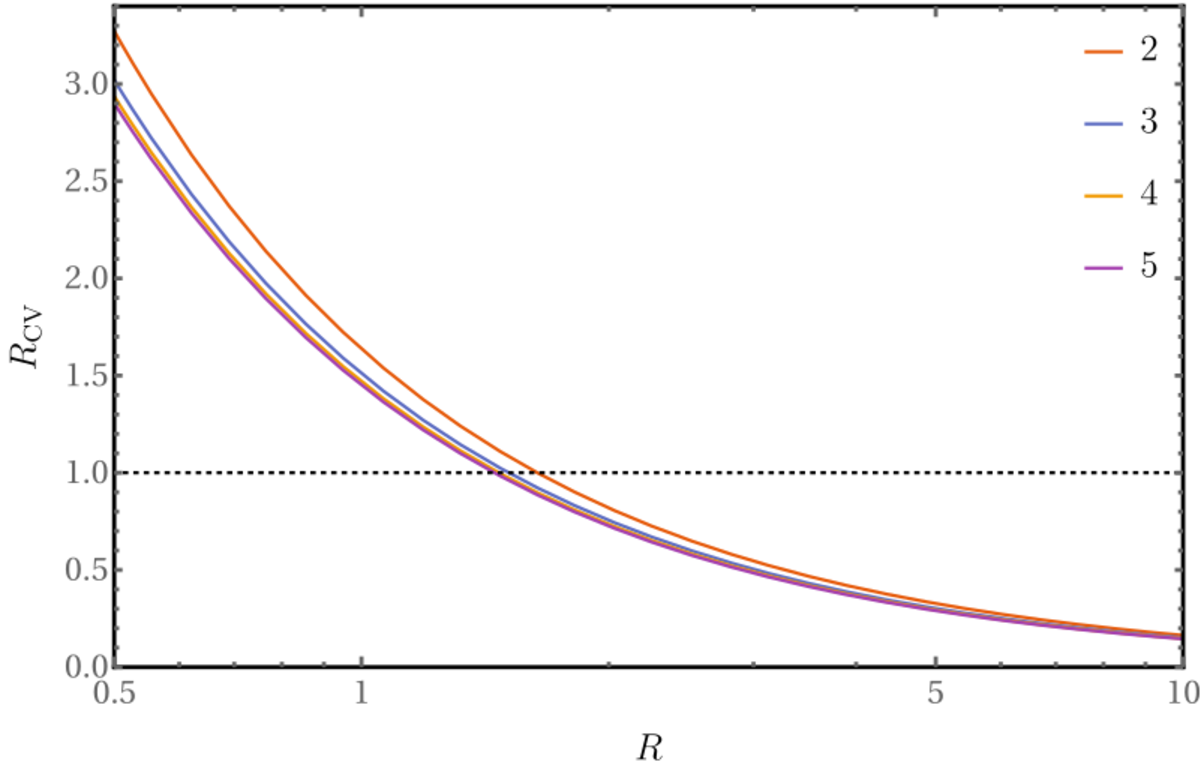
\includegraphics[width=0.49\textwidth]{WCElargebasis.pdf}
    \caption{Radius of convergence $R_{\text{CV}}$ in the CSF basis with $K$ basis functions for the MP (left) and WC (right) partitioning.}
    \label{fig:RadiusBasis}
\end{figure}

\begin{table}
\centering
\footnotesize
\caption{Dominant singularity in the CSF basis set ($K=8$) for various value of $R$ in the MP and WC partitioning.}
\begin{tabular}{cccccccc}
\hline
\hline
$R$ & 0.1 & 1 & 2 & 3 & 5 & 10 & 100 \\
\hline
MP & $+14.1-10.9\,i$ & $+2.38-1.47\,i$ & $-0.67-1.30\,i$ & $-0.49-0.89\,i$ & $-0.33-0.55\,i$ & $-0.22-0.31\,i$ & $+0.03-0.05\,i$ \\
WC & $-9.6-10.7\,i$ & $-0.96-1.07\,i$ & $-0.48-0.53\,i$ & $-0.32-0.36\,i$ & $-0.19-0.21\,i$ & $-0.10-0.11\,i$ & $-0.01-0.01\,i$ \\
\hline
\hline
\end{tabular}
\label{tab:SingAlpha}
\end{table}

\subsection{Exceptional points in the UHF formalism}\label{sec:uhfSing}

Now, we investigate the differences in the singularity structure between the RHF and UHF formalism. To do so, we use the symmetry-broken orbitals discussed in Sec.~\ref{sec:spherium}. Thus, the UHF two-electron basis is
\begin{align}\label{eq:uhfbasis}
 \psi_1 & =\phi_{\alpha,1}(\theta_1)\phi_{\beta,1}(\theta_2),
 & 
 \psi_2 & =\phi_{\alpha,1}(\theta_1)\phi_{\beta,2}(\theta_2),\\
 \psi_3 & =\phi_{\alpha,2}(\theta_1)\phi_{\beta,1}(\theta_2),
 & 
 \psi_4 & =\phi_{\alpha,2}(\theta_1)\phi_{\beta,2}(\theta_2).
\end{align}
with the symmetry-broken orbitals
\begin{subequations}
\begin{align}\label{eq:uhforbitals}
 	\phi_{\alpha,1}(\theta) 
 		& =\frac{\sqrt{75+62R}}{4\sqrt{7R}} Y_{0}(\theta)
 		+ \frac{5\sqrt{-3+2R}}{4\sqrt{7R}} Y_{1}(\theta),
 \\ 
 	\phi_{\beta,1}(\theta) 
		& =\frac{\sqrt{75+62R}}{4\sqrt{7R}} Y_{0}(\theta)
		- \frac{5\sqrt{-3+2R}}{4\sqrt{7R}} Y_{1}(\theta),
 \\
	 \phi_{\alpha,2}(\theta) 
	 & = - \frac{5\sqrt{-3+2R}}{4\sqrt{7R}} Y_{0}(\theta)
	  + \frac{\sqrt{75+62R}}{4\sqrt{7R}} Y_{1}(\theta),
 \\
	 \phi_{\beta,2}(\theta) 
	 & =\frac{5\sqrt{-3+2R}}{4\sqrt{7R}} Y_{0}(\theta)
	 +\frac{\sqrt{75+62R}}{4\sqrt{7R}} Y_{1}(\theta).
\end{align}
\end{subequations}

In the UHF formalism the Hamiltonian $\hH(\lambda)$ is no more block diagonal, $\psi_4$ can interact with $\psi_2$ and $\psi_3$. The matrix elements of the Hamiltonian corresponding to this interaction are
\begin{equation}\label{eq:MatrixElem}
	H_{24}=H_{34}=H_{42}=H_{43}=\sqrt{R-\frac{3}{2}}\sqrt{R+\frac{75}{62}}\qty(R+\frac{25}{2})\frac{\sqrt{31}}{70R^3}
\end{equation}

For $R=3/2$ the Hamiltonian is block diagonal because the matrix elements \eqref{eq:MatrixElem} are equal to zero so this is equivalent to the RHF case but for $R>3/2$ the matrix elements become real. This interaction corresponds to the spin contamination of the wave function. For $R<3/2$ the matrix elements are complex, this corresponds to the holomorphic solution of Fig.~\ref{fig:SpheriumNrj}, the singularities in this case will be treated later. The matrix elements become real again for $R<-75/62$, this corresponds to the sb-UHF solution for negative value of $R$ observed in Sec.~\ref{sec:spherium}. We will refer to the domain where the matrix elements are complex as the holomorphic domain.

The singularity structure in this case is more complex because of the spin contamination of the wave function. We can not use CSFs in this case. So when one compute all the degeneracies using Eqs.~\eqref{eq:PolChar} and \eqref{eq:DPolChar} some correspond to EPs and some correspond to conical intersections. The numerical distinction of those singularities is very difficult. We will first look at the energies $E(\lambda)$ obtained with this basis set to attribute a physical signification to the singularities obtained numerically.
Figure \ref{fig:UHFMiniBas} is the analog of Fig.~\ref{fig:RHFMiniBas} in the UHF formalism. We see that in this case the sp\textsubscript{z} triplet interacts with the s\textsuperscript{2} and the p\textsubscript{z}\textsuperscript{2} singlets. Those avoided crossings are due to the spin contamination of the wave function.

\begin{wrapfigure}{R}{0.5\textwidth}
    \centering
    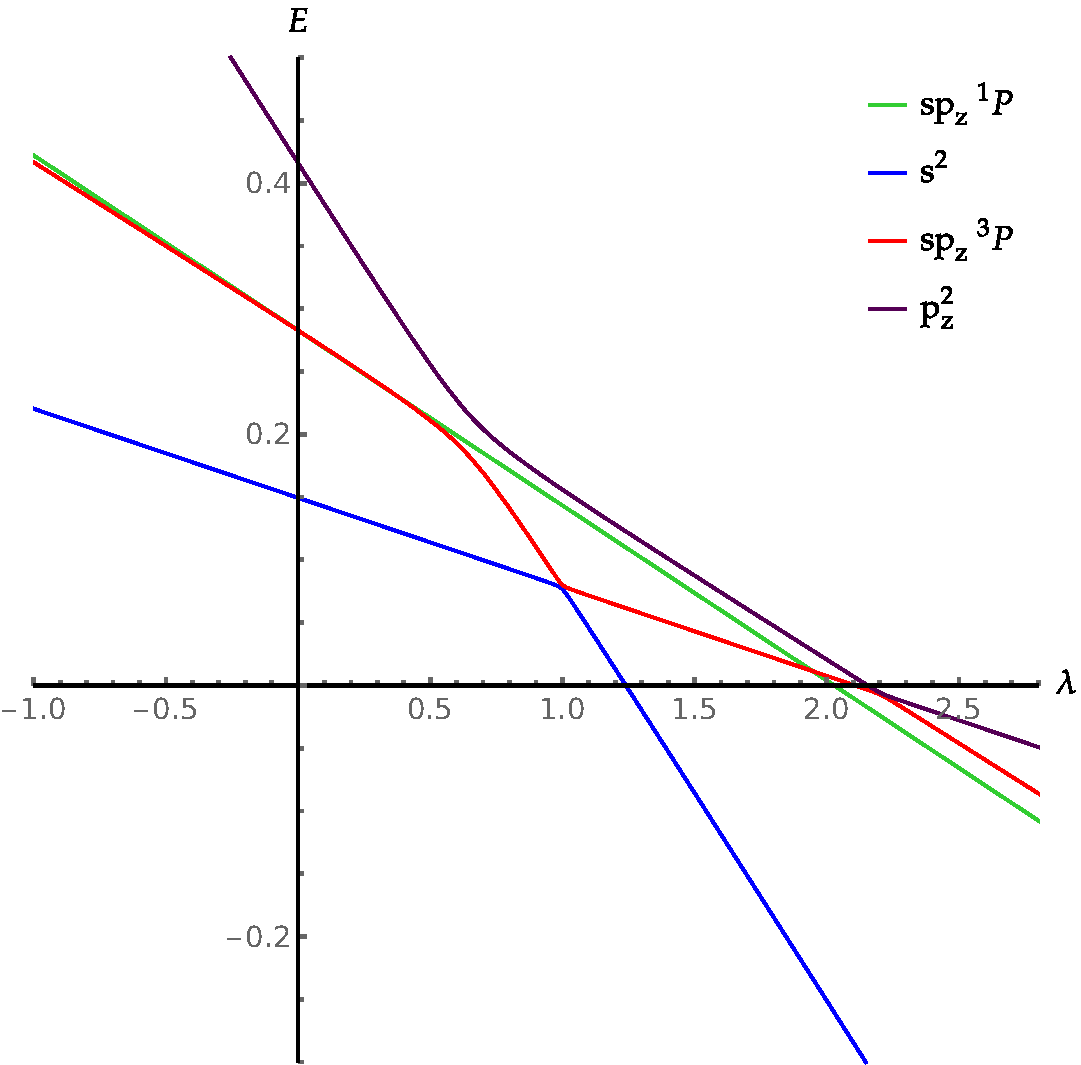
\includegraphics[width=\linewidth]{EMP_UHF_R10.pdf}
    \caption{Energies $E(\lambda)$ in the unrestricted basis set \eqref{eq:uhfbasis} with $R=10$.}
    \label{fig:UHFMiniBas}
\end{wrapfigure}

Within the RHF formalism, we have observed only $\alpha$ singularities and large avoided crossings but one can see in Fig.~\ref{fig:UHFMiniBas} that in the UHF case there are sharp avoided crossings which are known to be connected to $\beta$ singularities. For example at $R=10$ the pair of singularities connected to the avoided crossing between s\textsuperscript{2} and sp\textsubscript{z} $^{3}P$ is $0.999\pm0.014\,i$. And the one between sp\textsubscript{z} $^{3}P$ and p\textsubscript{z}\textsuperscript{2} is connected with the singularities $2.207\pm0.023\,i$. However, in spherium, the electrons cannot be ionized so those singularities cannot be the same $\beta$ singularities as the ones highlighted by Sergeev and Goodson \cite{Sergeev_2005}. We can see in Fig.~\ref{fig:UHFEP} that the s\textsuperscript{2} singlet and the sp\textsubscript{z} triplet states are degenerated for $R=3/2$. For $R>3/2$, it becomes an avoided crossing on the real axis and the degeneracies are $moved$ in the complex plane. The wave function is spin contaminated by $Y_1$ for $R>3/2$ this is why the s\textsuperscript{2} singlet energy cannot cross the sp\textsubscript{z} triplet curves anymore. When $R$ increases this avoided crossing becomes sharper. As presented before $\beta$ singularities are linked to quantum phase transition so it seems that this singularity is linked to the spin symmetry breaking of the UHF wave function. The fact that a similar pair of $\beta$ singularities appears for $R<-75/62$ confirms this assumption. The sharp avoided crossing between sp\textsubscript{z} $^{3}P$ and p\textsubscript{z}\textsuperscript{2} is not present on Fig. \ref{fig:UHFEP}. The second pair of $\beta$ singularities resulting from this avoided crossing appears for $R\gtrsim 2.5$, this is probably due to an excited-state quantum phase transition but this still need to be investigated. 

\begin{figure}
    \centering
    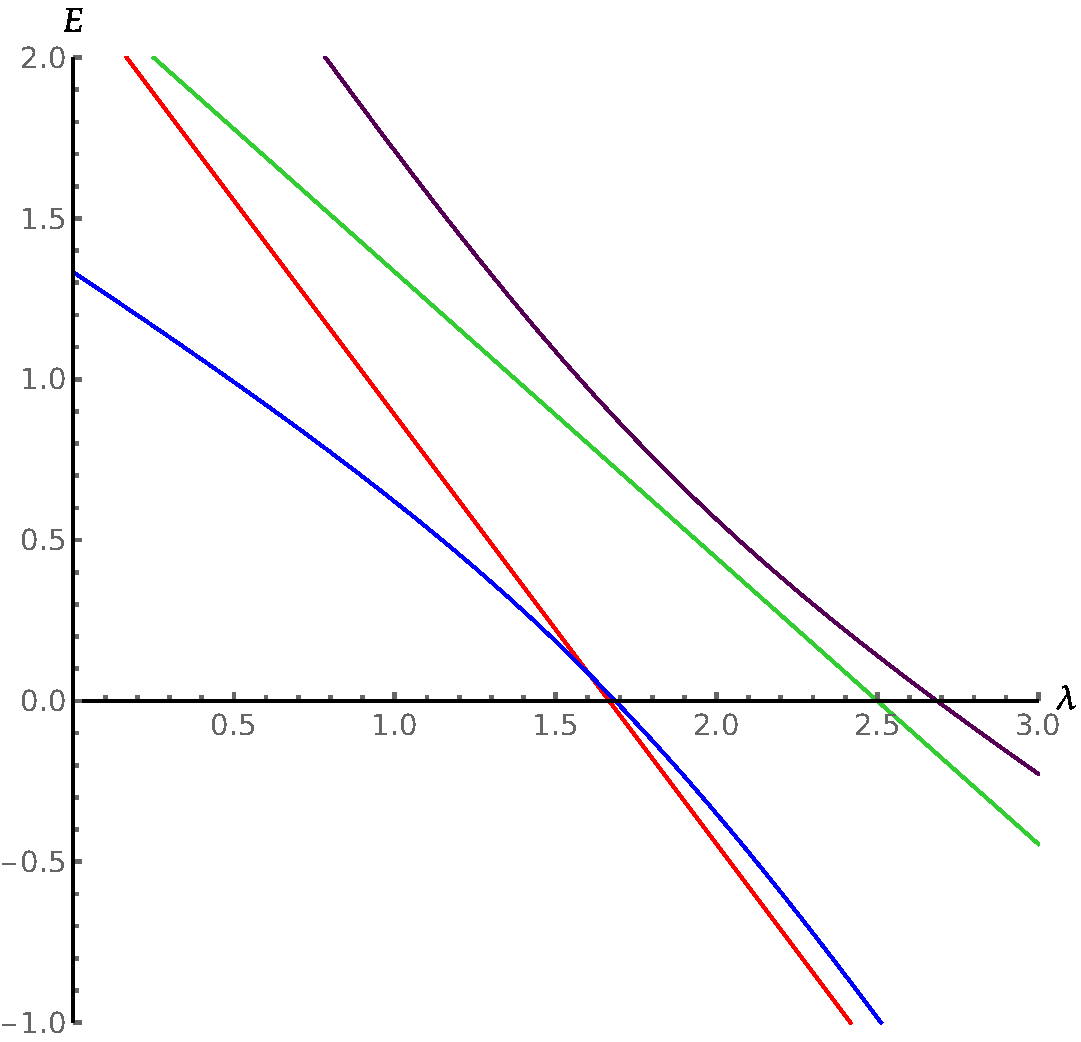
\includegraphics[width=0.45\textwidth]{UHFCI.pdf}
    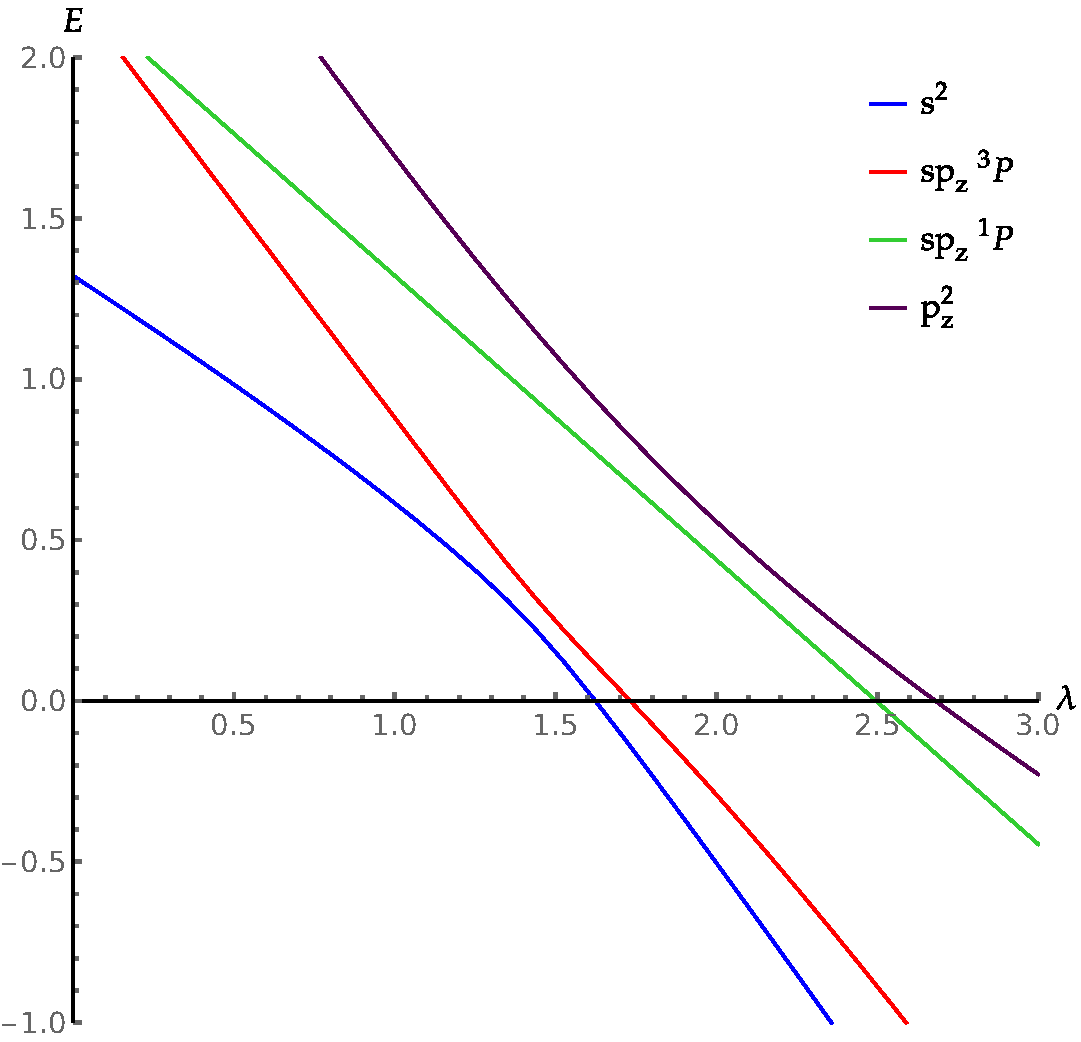
\includegraphics[width=0.45\textwidth]{UHFEP.pdf}
    \caption{Energies $E(\lambda)$ in the unrestricted basis set \eqref{eq:uhfbasis} for $R=1.5$ (left) and $R=1.51$ (right).}
    \label{fig:UHFEP}
\end{figure}

As shown before, some matrix elements of the Hamiltonian become complex in the holomorphic domain. Therefore the Hamiltonian becomes non-Hermitian for these values of $R$. In Ref.~\cite{Burton_2019a}, Burton \textit{et al.}~proved that for the \ce{H_2} molecule the unrestricted Hamiltonian is not \pt -symmetric in the holomorphic domain. An analog reasoning can be done with the spherium model to prove the same result. The \pt -symmetry (invariance with respect to combined space reflection $\mathcal{P}$ and time reversal $\mathcal{T}$) is a property which ensures that a non-Hermitian Hamiltonian has a real energy spectrum \cite{BenderBook}. Thus \pt -symmetric Hamiltonians can be seen as an intermediate class between Hermitian and non-Hermitian Hamiltonians.

Figure \ref{fig:UHFPT} shows that for the spherium model a part of the energy spectrum becomes complex when $R$ is in the holomorphic domain. The domain of values where the energy becomes complex is called the broken \pt-symmetry region. This is consistent with the fact that in the holomorphic domain the Hamiltonian is no more \pt -symmetric. 

For a non-Hermitian Hamiltonian the EPs can lie on the real axis. In particular, at the point of {\pt} transition (the point where the energies become complex) the two energies are degenerate resulting in such an EP on the real axis. This degeneracy can be seen in Fig.~\ref{fig:UHFPT}.

\begin{figure}[h!]
    \centering
    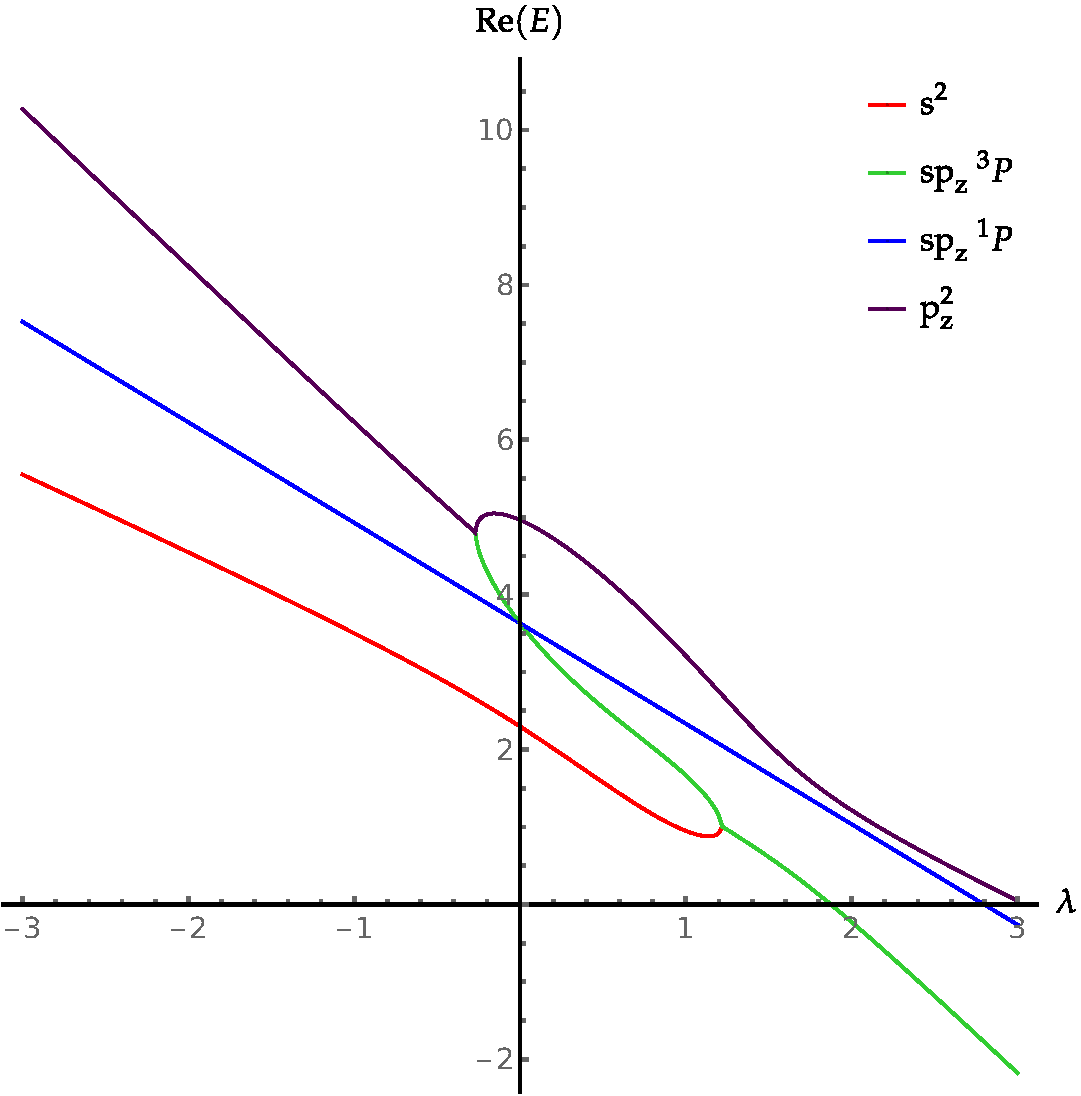
\includegraphics[width=0.45\textwidth]{ReNRJPT.pdf}
    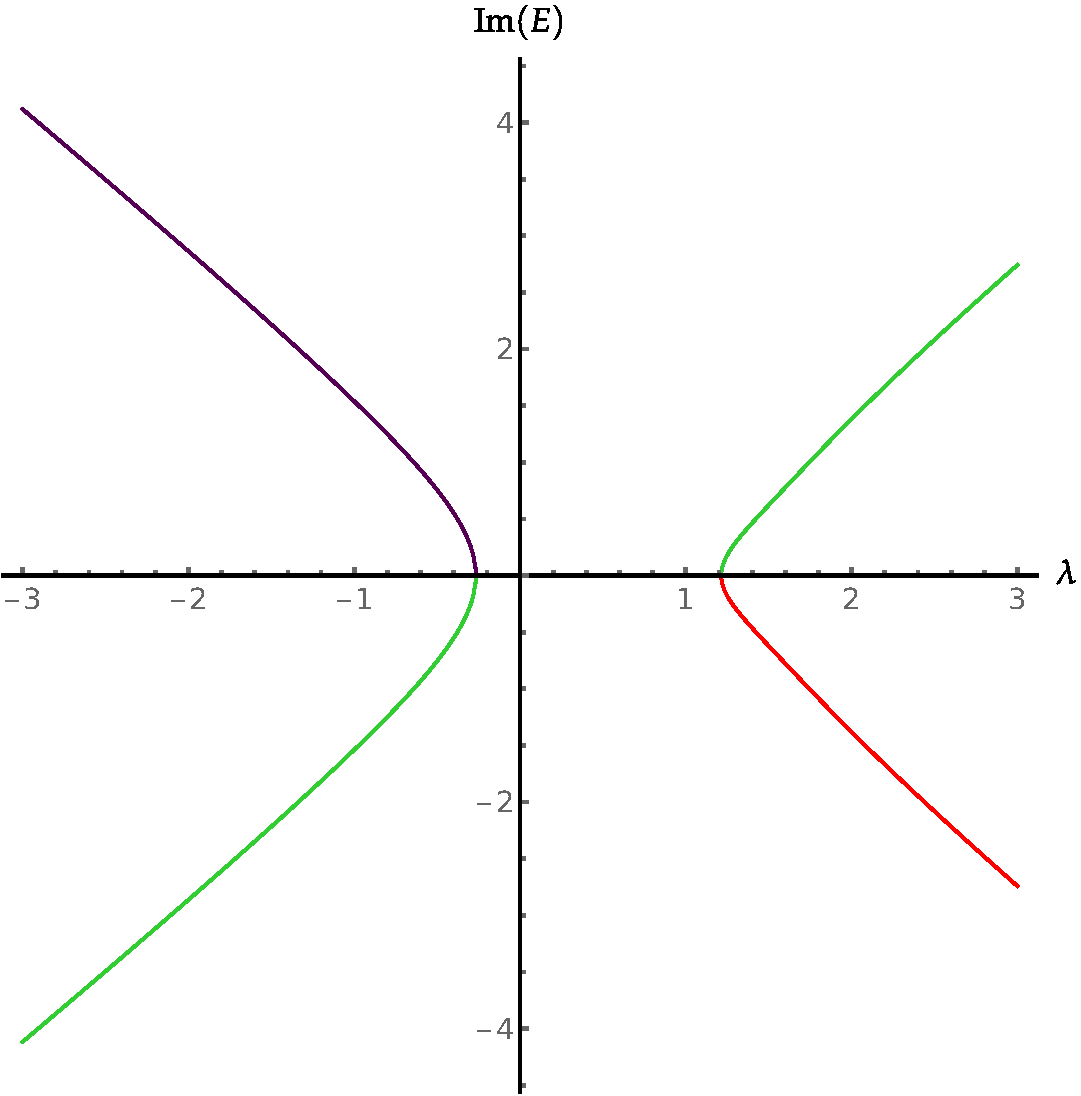
\includegraphics[width=0.45\textwidth]{ImNRJPT.pdf}
    \caption{\centering Real part (left) and imaginary part (right) of $E(\lambda)$ in the unrestricted basis set \eqref{eq:uhfbasis} for $R=1$.}
    \label{fig:UHFPT}
\end{figure}

\section{Conclusion}

In order to model accurately chemical systems, one must choose, in a ever growing zoo of methods, which computational protocol is adapted to the system of interest.
This choice can be, moreover, motivated by the type of properties that one is interested in.
That means that one must understand the strengths and weaknesses of each method, i.e., why one method might fail in some cases and work beautifully in others. 
We have seen that for methods relying on perturbation theory, their successes and failures are directly connected to the position of EPs in the complex plane. 
Exhaustive studies have been performed on the causes of failure of MP perturbation theory. 
First, it was understood that, for chemical systems for which the HF Slater determinant is a poor approximation to the exact wave function, MP perturbation theory fails too. Such systems can be, for example, molecules where the exact ground-state wave function is dominated by more than one configuration, i.e., multi-reference systems. 
More preoccupying cases were also reported. 
For instance, it has been shown that systems considered as well-understood (e.g., \ce{Ne}) can exhibit divergent behavior when the basis set is augmented with diffuse functions. 
Later, these erratic behaviors of the perturbation series were investigated and rationalized in terms of avoided crossings and singularities in the complex plane. It was shown that the singularities can be classified in two families. 
The first family includes $\alpha$ singularities resulting from a large avoided crossing between the ground state and a low-lying doubly-excited states. 
The $\beta$ singularities, which constitutes the second family, are artifacts generated by the incompleteness of the Hilbert space, and they are directly connected to an ionization phenomenon occurring in the complete Hilbert space. 
These singularities are close to the real axis and connected with sharp avoided crossing between the ground state and a highly diffuse state. 
We have found that the $\beta$ singularities modeling the ionization phenomenon described by Sergeev and Goodson are actually part of a more general class of singularities. Indeed, those singularities close to the real axis are connected to quantum phase transition and symmetry breaking, and theoretical physics have demonstrated that the behavior of the EPs depends of the type of transitions from which the EPs result (first or higher orders, ground state or excited state transitions).

In this work, we have shown that $\beta$ singularities are involved in the spin symmetry breaking of the UHF wave function. 
This confirms that $\beta$ singularities can occur for other types of transition and symmetry breaking than just the formation of a bound cluster of electrons. 
It would be interesting to investigate the difference between the different type of symmetry breaking and how it affects the singularity structure. 
Moreover the singularity structure in the non-Hermitian case still need to be investigated. 
In the holomorphic domain, some singularities lie on the real axis and it would also be interesting to look at the differences between the different symmetry breaking and their respective holomorphic domain. 
Furthermore, in this study we have used spherical harmonics (or combination of spherical harmonics) as basis functions which have a delocalized nature. It would also be interesting to investigate the use of localized basis functions \cite{Seidl_2018} (for example gaussians) because these functions would be more adapted to describe the strongly correlated regime. %More generally, to investigate the effect of the type of basis on the physics of EPs.
To conclude, this work shows that our understanding of the singularity structure of the energy is still incomplete but we hope that it opens new perspectives for the understanding of the physics of EPs in electronic structure theory.



\newpage
\printbibliography


\end{document}
